% hello
\documentclass{article}

\usepackage[utf8]{inputenc}
\usepackage{graphicx}
\usepackage[dvipsnames]{xcolor}
\usepackage{csquotes}
\usepackage{hyperref}
\usepackage{tabularx}
\usepackage{booktabs}
\usepackage{pdfpages}
\usepackage{caption,geometry}
\usepackage[toc,page]{appendix}
\newcommand\myshade{85}
\colorlet{mylinkcolor}{violet}
\colorlet{mycitecolor}{YellowOrange}
\colorlet{myurlcolor}{Aquamarine}

\hypersetup{
  linkcolor  = mylinkcolor!\myshade!black,
  citecolor  = mycitecolor!\myshade!black,
  urlcolor   = myurlcolor!\myshade!black,
  colorlinks = true,
}

\usepackage[acronym]{glossaries}

\usepackage{listings}
\lstset{
    frame=Trbl,
    numbers=left,
    breaklines=true,
    basicstyle=\ttfamily,
    postbreak=\mbox{\textcolor{red}{$\hookrightarrow$}\space}
}

\usepackage[maxnames=3,style=authoryear,natbib=true]{biblatex}
\addbibresource{./references.bib}
% \bibliographystyle{unsrtnat}
% \setcitestyle{authoryear}


\newglossary[bsg]{bus}{bsd}{bsn}{Bussiness glossary}
\newglossary[dmg]{dm}{dmd}{dmn}{Data mining glossary}

\graphicspath{ {../images/} }

\DeclareUnicodeCharacter{2008}{-}% support older LaTeX versions
\DeclareUnicodeCharacter{2003}{ }% support older LaTeX versions

\let\oldautoref\autoref
\renewcommand{\autoref}[1]{(\oldautoref{#1})}
\newcommand{\autorefsub}[2]{(\oldautoref{#1}, #2)}
\newcommand{\gmt}{\acrshort{gmt}}
\newcommand{\firstvis}{first-visit data }
\newcommand{\secondvis}{second-visit data }

\newcommand{\uu}{Utrecht University}
\newcommand{\flup}{\gls{d:flup} }
\newcommand{\simon}{\gls{d:simon} }
\newcommand{\dpaper}{the \flup paper }
\newcommand{\Dpaper}{The \flup paper }
\newcommand{\spaper}{the \simon paper }

\newcommand{\MyTitle}[1]{
    \title{
    {#1}\\
    {\large Utrecht University}\\
    }
    \author{Mike Vink}
    \date{ \today }
    \maketitle
}
\newcommand{\f}[3]{%
\begin{figure}[htpb]
    \includegraphics[width=\textwidth]{#1}
    \caption{#2}
    \label{#3}
\end{figure}
}

\newcommand{\fptable}[5]{%

\newgeometry{scale=1}
\thispagestyle{empty}

\begin{table}
{%
    \centering
    \includegraphics[scale=.7]{#1}
    \captionsetup{width=0.8\linewidth}
    \captionof{table}{\textbf{#3} #4}
    \par
    \label{#5}
}
\end{table}

\restoregeometry
}

\newcommand{\fpfig}[5]{%

\newgeometry{scale=1}
\thispagestyle{empty}

\begin{figure}
{%
    \centering
    \includegraphics[scale=.7]{#1}
    \captionsetup{width=0.8\linewidth}
    \captionof{figure}{\textbf{#3} #4}
    \par
    \label{#5}
}
\end{figure}

\restoregeometry
}



\makeglossaries
\newglossaryentry{bu:rnaVirus}
{
    type=bus,
    name=ribonucleic acid virus(es),
    description={An \acrshort{rna} virus is a virus that has \acrshort{rna} as
    its genetic material. Inside a host cell this material is used to generate
    new virusses. Notable human diseases caused by RNA viruses include the
    common cold and influenza}
}
\newglossaryentry{bu:antigen}
{
    type=bus,
    name=antigen,
    description={In immunology, an antigen is a molecule or molecular
    structure, such as \acrshort{ha} and \acrshort{na}, that can be bound by an
    antigen-specific \gls{bu:antibody} or immune cell receptor.  The presence of
    antigens in the body normally triggers an immune response
    }
}
\newglossaryentry{bu:glycoprotein}
{
    type=bus,
    name=glycoprotein,
    description={Glycoproteins are molecules that comprise protein and
    carbohydrate chains. Many viruses have external glycoproteins that
    help them enter bodily cells, but can also serve to be important
    therapeutic or preventative targets}
}
\newglossaryentry{bu:mutation}
{
    type=bus,
    name=mutation,
    description={Mutation of genetic material occurs thanks to its chemical
    instability. The encoded protein molecules can have single amino acid
    (protein building block) change (minor, but still in many cases significant
    change leading to disease) or wide-range amino acid changes}
}
\newglossaryentry{bu:tiv}
{
    type=bus,
    name=TIV,
    description={
        An inactivated trivalent vaccine is a vaccine consisting of \gls{bu:antigen}ic virus particles from viruses that have been grown in culture and then killed to destroy disease producing capacity.
        In practice vaccines of three main types of influenza were used, hence trivalent
    },
    first={inactivated trivalent vaccines (TIV)}
}
\newglossaryentry{bu:antibody}
{
    type=bus,
    name=antibody,
    description={ Protein used by the immune system to identify and neutralize foreign objects such as pathogenic bacteria     and viruses.
    The antibody recognizes a unique molecule of the pathogen, called an \gls{bu:antigen}}
}
\newglossaryentry{bu:titer}
{
    type=bus,
    name=titer,
    description={
    Titer is a way of expressing concentration.
    Titer testing employs serial dilution to obtain approximate quantitative information from an analytical procedure that inherently only evaluates as positive or negative.
    The titer corresponds to the highest dilution factor that still yields a positive reading
    }
}
\newglossaryentry{bu:tcell}
{
    type=bus,
    name=T-cell,
    description={
        A T cell is a type of \gls{bu:lymphocyte}.
        T cells are one of the important white blood cells of the immune system and play a central role in the adaptive immune response, for example generating antibodies against influenza.
        Groups of specific, T cell subtypes have a variety of important functions in controlling and shaping the adaptive immune response
    }
}
\newglossaryentry{bu:lymphocyte}
{
    type=bus,
    name=lymphocyte,
    description={
        A lymphocyte is a type of white blood cell in the immune system of jawed vertebrates.
        Lymphocytes include \gls{bu:tcell}, and \gls{bu:bcell}.
        These cells work together in the adaptive immune response to generate antibodies against influenza
    }
}
\newglossaryentry{bu:cd8pos}
{
    type=bus,
    name=CD8+ T-cell,
    description={
        A cytotoxic T cell (also known as CD8+ T-cell) is a \gls{bu:tcell} that kills cancer cells, cells that are infected (particularly with viruses), or cells that are damaged in other ways.
        It does so by recognizing specific part of \gls{bu:antigen} and then starting a process that kills the targetted cell
    }
}
\newglossaryentry{bu:cd4pos}
{
    type=bus,
    name=CD4+ T-cell,
    description={
        The T helper cells, also known as CD4+ cells, "help" the activity of other immune cells by releasing \gls{bu:cytokine}s.
        These cells help to polarize the immune response into the appropriate kind depending on the nature of the immunological insult (e.g. virus vs. bacterium)
    }
}
\newglossaryentry{bu:cytokine}
{
    type=bus,
    name=cytokine,
    description={
        Cytokines are a broad and loose category of small proteins important in cell signaling that bind to receptor protein on the outside of (immune) cells to fulfill their signal function
    }
}
\newglossaryentry{bu:pbmc}
{
    type=bus,
    name=PBMC,
    description={
        A peripheral blood mononuclear cell is any peripheral blood cell having a round nucleus.
        These cells consist of \gls{bu:lymphocyte} and \gls{bu:monocyte}s
    },
    first={peripheral blood mononuclear cell (PBMC)}
}
\newglossaryentry{bu:bcell}
{
    type=bus,
    name=B-cell,
    description={
        B-cells produce antibody molecules; however, these antibodies are not secreted.
        Rather, they are presented on the outside of the cell where they serve as a part of B-cell receptors.
        When a B-cell is activated by an antigen, it proliferates and differentiates into an antibody-secreting effector cell, known as a plasmablast or plasma cell
    }
}
\newglossaryentry{bu:monocyte}
{
    type=bus,
    name=monocyte,
    description={
        Monocytes are a type of white blood cell.
        Monocytes and their macrophage and dendritic cell progeny serve three main functions in the immune system.
        These are phagocytosis, antigen presentation, and cytokine production.
        Phagocytosis is the process of uptake of microbes and particles followed by digestion and destruction of this material
    }
}
\newglossaryentry{bu:hai}
{
    type=bus,
    name=HAI,
    description={
        The \acrlong{ha} inhibition assay is used to measure the \gls{bu:titer} of \gls{bu:antibody} against a strain of influenza virus present in the serum.
        Antibody levels are measured before vaccination and 28 days after.
        The antibody levels are used to compute the seroprotection and seroconversion criteria
    },
    first={\acrlong{ha} inhibition assay (HAI)}
}
\newglossaryentry{bu:cmv}
{
    type=bus,
    name=CMV,
    description={
        Cytomegalovirus (CMV) is a common herpesvirus found in humans.
        Like other herpesviruses, it is a life-long infection that remains in a latent state inside the human body, until it is 'reactivated' by appropriate conditions.
        Thought to accelerate aging of the immune system and thereby impairing influenza vaccine response  \citep{van_den_Berg_2019}
    },
    first={cytomegalovirus (CMV)}
}
\newglossaryentry{bu:ebv}
{
    type=bus,
    name=EBV,
    description={
        The Epstein–Barr virus (EBV), is one of the nine known human herpesvirus types in the herpes family, and is one of the most common viruses in humans.
    },
    first={Epstein-Barr virus (EBV)}
}
\newglossaryentry{bu:seropc}
{
    type=bus,
    name=seroconversion and seroprotection,
    description={
        A vaccine is considered succesful if the recipient seroconverted (4-fold or greater rise in antibody against virus after vaccination) and were seroprotected (\acrshort{gmt} \(\ge\) 40) after vaccination.
    }
}
\newglossaryentry{bu:stat}
{
    type=bus,
    name=STAT,
    description={
        A vaccine is considered succesful if the recipient seroconverted (4-fold or greater rise in antibody against virus after vaccination) and were seroprotected (\acrshort{gmt} \(\ge\) 40) after vaccination.
    },
    first={signal transducers and activators of transcription (STAT)}
}



\newglossaryentry{d:model}
{
    type=dm,
    name=model,
    description={model is a model}
}
\newglossaryentry{d:flup}
{
    type=dm,
    name=FluPrint,
    description={Data used in this work}
}
\newglossaryentry{d:simon}
{
    type=dm,
    name=SIMON,
    description={Follow up study used in this work}
}

\newacronym{ha}{HA}{hemagglutinin}
\newacronym{na}{NA}{neuraminidase}
\newacronym{rna}{RNA}{ribonucleic acid}


\begin{document}
\MyTitle{Change in immune cell signaling upon repeat vaccination: a data exploration using the FluPrint database}
\tableofcontents
\printglossary[type=bus]
\printglossary[type=dm]
\printglossary[type=\acronymtype]


\section{background}

Influenza viruses are enveloped \gls{bu:rnaVirus} (\acrshort{rna} virus(es)) and
are divided into three types on the basis of \gls{bu:antigen}ic differences of internal
structural proteins \citep{fdaGuidanceIndustryClinical2007}.

Two influenza virus types, Type A and B, cause yearly epidemic outbreaks in humans
and are further classified based on the structure of two major external
\gls{bu:glycoprotein}s, hemagglutinin (\acrshort{ha}) and neuraminidase (\acrshort{na})
\citep{fdaGuidanceIndustryClinical2007}.

Type B viruses, which are largely restricted to the human host, have a single
\acrshort{ha} and \acrshort{na} subtype.  In contrast, numerous \acrshort{ha}
and \acrshort{na} Type A influenza subtypes have been identified to date.  Type
A and B influenza variant strains emerge as a result of frequent
\gls{bu:antigen}ic change, principally from \gls{bu:mutation}s in the \acrshort{ha}
and \acrshort{na} \gls{bu:glycoprotein}s \citep{fdaGuidanceIndustryClinical2007}.

Since 1977, influenza A virus subtypes H1N1 and H3N2, and influenza B viruses
have been in global circulation in humans. The current U.S. licensed
\gls{bu:tiv} are formulated to prevent influenza illness
caused by these influenza viruses.  Because of the frequent emergence of new
influenza variant strains, the \gls{bu:antigen}ic composition of influenza vaccines
needs to be evaluated yearly, and the \gls{bu:tiv} are reformulated almost every
year.

Currently, even with full production, manufacturing capacity would not produce
enough seasonal influenza vaccine to vaccinate all those for whom the vaccine
is now recommended \citep{fdaGuidanceIndustryClinical2007}.

\subsection{Influenza mortality estimation models}

Numerous works apply regression models to describe seasonal population
influenza mortality \citep{zhouHospitalizationsAssociatedInfluenza2012,
greenMortalityAttributableInfluenza2013, iulianoEstimatesGlobalSeasonal2018}.
Reported are varying age-specific influenza burdens during different seasonal
epidemics for different regions, but in general young children an elderly are
found to be more susceptible to influenza and are adviced to vaccinated
annually \citep{zhouHospitalizationsAssociatedInfluenza2012}.

Specifically, within the US based work of
\cite{zhouHospitalizationsAssociatedInfluenza2012}, the highest hospitalization
rates for influenza were among persons aged $>=$65 years and those aged $<$1
year.  And, age-standardized annual rates per 100000 person-years varied
substantially for influenza. A similar pattern is in
\cite{greenMortalityAttributableInfluenza2013}, where an age shift in Wales and
England seasonal influenza burden was observed following the 2009 swine flue
pandemic. It is also estimated that globally 291.243–645.832 influenza associated
seasonal deaths occur annually \citep{iulianoEstimatesGlobalSeasonal2018} These
varying demographic statistics and the volume of influenza patients can confound
decision making on national and international public health policies.
Knowledge on vaccine efficacy and implementation can be a valuable asset for
fighting future seasonal influenza outbreaks.

\subsection{Vaccine success criteria}

Due to the volume and vulnerability of population groups most at risk for
influenze, the young and the elderly, a placebo controlled vaccine efficacy
study is extremely costly \citep{zhouHospitalizationsAssociatedInfluenza2012}.
Instead the haemagglutination-inhibiting (HAI) antibody test for influenza
virus antibody is used to assess vaccine protection
\citep{dejongHaemagglutinationinhibitingAntibodyInfluenza2003}. The policy for
a succesful vaccine is an 4-fold increase in HAI antibody titre after
vaccination and a geometric mean HAI titer of $\geq$ 40. The last is predicted
to reduce influenza risk by 50\%
\cite{dejongHaemagglutinationinhibitingAntibodyInfluenza2003}.

\subsection{Finding immunological factors predicting high vaccine response using machine learning}

It is known that pre-existing T cell populations are correlated with a HAI
antibody response after vaccination. But, the role of T cells in mediating that
response is uncertain. In one work it was found that under certain
circumstances CD8+ T cells specific to conserved viral epitopes correlated with
protection against symptomatic influenza
\citep{sridharCellularImmuneCorrelates2013}.In other work, populations of CD4+
T cells that associated with protective antibody responses after seasonal
influenza vaccinations were found \citep{bentebibelInductionICOSCXCR3}.
\cite{trieuLongtermMaintenanceInfluenzaSpecific2017} reports a stable CD8+ T
cell populations and an increased CD4+ T cell populatin after vaccination. It was
also reported that repeat vaccinations are an important factor in maintaining
CD4+ T cell population \citep{trieuLongtermMaintenanceInfluenzaSpecific2017}.
How exactly these T cell populations factor into protective influenza immunity
and vaccination reponse is not well understood.

Machine learning has been applied to clinical datasets to find influenza
protection markers, such as the described T cell populations and titers of
related molecules \citep{furmanApoptosisOtherImmune2013,
sobolevAdjuvantedInfluenzaH1N1Vaccination2016, tsangGlobalAnalysesHuman2014}.
These type of studies suffer from data quality issues, such as: inconsistencies
between findings depending on the epidemic season, only focussing on one type
of biological assay to get data, and a low amount of patients/samples. A
succesful vaccination is also often not well defined.

\subsection{Bussiness objectives}

Due to the high volume population that needs vaccines, it is important to study
immune correlates to vaccine response. For example, repeat vaccination might
not be necessary if the response is low, or a different vaccine is desired on a
person to person basis depending on immune correlates. Moreover, identifying
patterns between vaccine response and immune correlates furthers the
understanding of the underlying immunological mechanism of influenza
protection.

This work uses the \flup database, which aims to solve data quality issues
and low dimensionality of prior studies using clinical datasets comprised of
viurs, cell and serum sample assays. It does so by incorporating eigth clinical
studies conducted between 2007 to 2015 using in total 740 patients, including
different types of assays and normalizing their values, and by providing a
binary classification of high- and low-responder to a vaccine.

The objectives of this work are to answer:
\begin{itemize}
        \item What kind of studies can be done using the \flup database?
        \item What immunological factors correlate to a vaccine responses?
        \item What is the effect of repeat vaccination?
\end{itemize}

Since this work is an independent study performed for an assignment, the
success criteria for these objective will be loosely defined as providing a
statistical description or to provide insigth in the questions posed in the
objectives.

The rationale for these questions and succes criteria  are based on the scope
of the 3EC project as part of the Applied data science profile and the data
available. The paper of \cite{tomicFluPRINTDatasetMultidimensional2019} on
which this work is mostly based on provides these questions as interesting
directions for further analysis, but does not directly provide the data
necessary to answer them, only the MySQL database containing a great volume of
data.

\section{Assess situation}

\subsection{data and knowledge sources}

The sole source of data used in the project is provided by
\cite{tomicFluPRINTDatasetMultidimensional2019} (this work is reffered to
using: "the \flup paper" from now on). \Dpaper describes the MySQL database for
which the installation is described in the
\href{https://github.com/LogIN-/fluprint}{FluPrint Github Repository}. A
template query is provided on the
\href{https://github.com/LogIN-/simon-manuscript}{github page} belonging to an
unpublished follow-up study by the same authors of \dpaper
\autoref{lst:QueryTemplate}.  According to the authors, this data is the most
interesting for the bussiness objective of finding repeat vaccination effects
and will be used in this work too (this
unpublished follow-up study is referred to using: "\spaper"). The authors give this brief
description of the data:

\begin{displayquote}
    \textit{"The influenza datasets were obtained from the Stanford Data Miner maintained by
    the Human Immune Monitoring Center at Stanford University. This included
    total of 177 csv files, which were automatically imported to the MySQL
    database to facilitate further analysis. The database, named \flup and
    its source code, including the installation tutorial are freely available
    here and on project's website. Following database installation, you can
    obtain data used in the SIMON publication by following MySQL database
    query \autoref{lst:QueryTemplate}"}.
\end{displayquote}

\subsection{Tools and techniques}

Installation of the \flup database will require an installation on a
unix operating system of \href{https://www.mysql.com/}{MySQL},
\href{https://www.php.net/manual/en/install.php}{PHP}. More details are at the
\href{https://github.com/LogIN-/fluprint}{FluPrint Github Repository}.

Database querying was done using a \href{https://neovim.io/}{neovim} based toolset,
personal configuration can be found
\href{https://github.com/Vinkage/mike_neovim/tree/feature}{here}.

Since in \dpaper R is used, it is also used here.  Especially crucial is the
\href{https://cran.r-project.org/web/packages/mulset/index.html}{R package
mulset}, which was made by the authors of \spaper. This package is used to deal
with missing data between different clinical studies and years, and thus will
be used to generate complete data tables in this paper too. All scripts in this
work were written using \href{https://www.tidyverse.org/}{tidyverse} packages
and make heavy use of the \href{https://dplyr.tidyverse.org/}{dplyr} package
for data wrangling. Additionally the following packages were used:
\href{https://cran.r-project.org/web/packages/ggpubr/index.html}{ggpubr} for
making publication quality figures, the kable function from
\href{knitr}{https://www.r-project.org/nosvn/pandoc/knitr.html} to generate
latex tables, \href{https://topepo.github.io/caret/}{caret} and
\href{https://cran.r-project.org/web/packages/MLeval/index.html}{MLeval} to
streamline model training and evaluation,
\href{https://cran.r-project.org/web/packages/corrplot/vignettes/corrplot-intro.html}{corrplot}
to visualise correlation between features, and other packages that were used
only once.

\subsection{Requirements of the project}

Requirements of this work are to show ability in using data science methods.
As such, most of the insights will inevitably be a replication of the work done
by the authors of the FluPrint database \cite{tomicSIMONAutomatedMachine2019},
but all the scripts and analysis done are original work and are supplied
together with the final deliverable.

Since the data type used here is a database this makes it more complicated for
an examinator to reproduce all code, especially since installing the database
requires a unix operating system. This is not considered problematic
since the queried tables from the database will be included in the final
deliverable.

Reporting of the project follows the CRISP-DM methodology, where at each
stage of the project a separate report is written during the analysis work. In
the end the most important information is kept and incorporated in a final
report that is assumed to be graded in conjunction with the code.

\subsection{Assumptions of the project}

This work assumes that the focus point of the evaluation lies on the
methodology used, and the ability to apply the basic data science methods
learned in the Applied Data Science profile. The answer to business objectives
is assumed to be subjective, and it is assumed that the methods used and
clarity of insights into the data gained are more important.

It is also assumed that the FluPrint database and other methods used by the
authors \cite{tomicFluPRINTDatasetMultidimensional2019,
tomicSIMONAutomatedMachine2019} are of high quality, and that this is
appropriate for this work. Out of the scope of this work is investigating
whether the preprocessing done for the data in the database is valid, since we
are not domain experts. A method for querying, cleaning, and generating
complete data tables has been provided by the authors and will also be used in
this work. It is assumed that the SQL and R methods (in particular the mulset R
package) in question are allowed to be used as a starting point in this
assignment.

\subsection{Constraints of the project}

This work is an unsupervised assignment, and only personal hardware were
available. This put constraints on dataset size and computational requirements
of analyses. The work was done on a Macbook air (2017) with the OSX big-sur
operating system. This means that unix tools were available and there were no
technical constraints. The filetypes are only csv files generated by the SQL
server.

\section{Data mining goals}

\subsection{Translating the problem in data mining terms}
All bussiness objectives described involve querying data from the FluPrint
database. The goal of the authors of the FluPrint database was to provide a
unqiue opportunity to study immune correlates of high vaccine responders across
different years and clinical studies. The authors also provide a binary
classification for donors. In this work we first and foremost explore the
database, and lastly we apply feature selection methods and classification
models on the most interesting dataset.

The bussiness objectives can be translated in data mining terminology like so:
\begin{itemize}
        \item Explore and describe the database and corresponding tables.
        \item Apply wrapper feature selection to the most interesting datasets.
        \item Explore features identified by the models trained in the wrapper feature selection.
\end{itemize}

In data mining terms, the problem type is a combination of exploratory data
analysis and classification. Since this work is for a 2-weeks/3EC assignment
for the Applied Data Science profile, success criteria for all goals are
subjective. For the classification type goals we follow
the model evaluation procedure used by the authors
\cite{tomicSIMONAutomatedMachine2019}, models were evaluated by the AUROC
metric, and accuracy, specificity and sensitivity were also reported. Insights
produced by this work were benchmarked against the work of the original
authors.

\subsection{Project plan}

\f{v2_desc_exploration}
{Project plan for the SQL related data mining goal.}
{plan:sql}

The first part of the project involved querying the database, and collecting
and describing the available data \autoref{plan:sql}. The first goal is to
understand the tables in the SQL database, their key relations, and to describe
the attributes within the tables. Valuable info on this part is already
provided in the original publication of the database
\cite{tomicFluPRINTDatasetMultidimensional2019}, but it was also investigated
in this work. The tools that will be used are SQL for querying and R for
statistical descriptions.

% The second phase of this plan was an iterative process of finding suitable data
% to answer the modeling and visualisation data mining goals. This is a more
% involved process since it requires exploration of the database to answer the
% questions, and therefore was estimated to take time.

% \f{model_and_vis_plan}
% {Project plan for the modeling and visualisation data mining goals.}
% {plan:vis}
%
% Relations between attributes in the generated datasets are visualised and
% modelled to see if there exist a pattern in the data that is relevant for the
% business objectives \autoref{plan:vis}. A critical point in this plan is
% deciding whether an objective cannot be answered with the available data. In
% that case the goal was revised and the second phase of the SQL query plan was
% reiterated. When deciding if the exploratory analysis was of sufficient
% quality, the work by the authors of the database used in this work was used as
% a subjective benchmark \cite{tomicSIMONAutomatedMachine2019,
% tomicFluPRINTDatasetMultidimensional2019}.

\f{feature_selection_classification}
{Project plan for the classification and feature selection data mining goal.}
{plan:cls}

For the modeling data mining goals the plan was to find the immune correlates
of high immune responders using a wrapper based feature selection strategy
\autoref{plan:cls}


\section{Data description}

\subsection{Volumetric analysis}

In the work of \cite{tomicFluPRINTDatasetMultidimensional2019} data on
indiviuals enrolled in influenza vaccine studies at the Stanford-LPCH Vaccine
Program was collected, the data was archived at the Stanford Data Miner. This
archive was filtered by assays used in influenza studies, resulting in data
from 740 healthy donors, enrolled in influenza vaccine studies conducted by the
Stanford-LPCH Vaccine Program from 2007 to 2015. These studies are described in
the table accompanying the online publication of the fluprint dataset
\autoref{tbl:studiesDesc}.  From those 740 donors a vaccine response
classification was only given for 372 donors \autoref{fig:demoGraph}, by a
method that will be described in the section describing the data table
containing this attribute. Overall there was no major difference in demographic
statistics when stratisfying the data in high or low responder classification
\autoref{fig:demoGraph}.

Importantly, it is reported that in all studies the donors are only vaccinated
once, except in the study SLVP015 \autoref{tbl:studiesDesc}
\citep{tomicFluPRINTDatasetMultidimensional2019}. However, in later work of the
same authors it is claimed that vaccines are administered as specified by the study
\citep{tomicSIMONAutomatedMachine2019}.

The donors for which a vaccine respone classification was available from all
clinical studies together span a wide age range \autoref{fig:demoGraph}A from 1
- 50 \autoref{tbl:demoStats}, in the original work the demographic statistics
include the donors for which no vaccine response classification is given,
therefore they report a greater range of 1-90. Stratisfying the donors on
vaccine response does not affect the demographic attribute distribution, but
the maximum age is lowered in the high responders group
\autoref{fig:demoGraph}B.

\begin{figure}[htpb]
    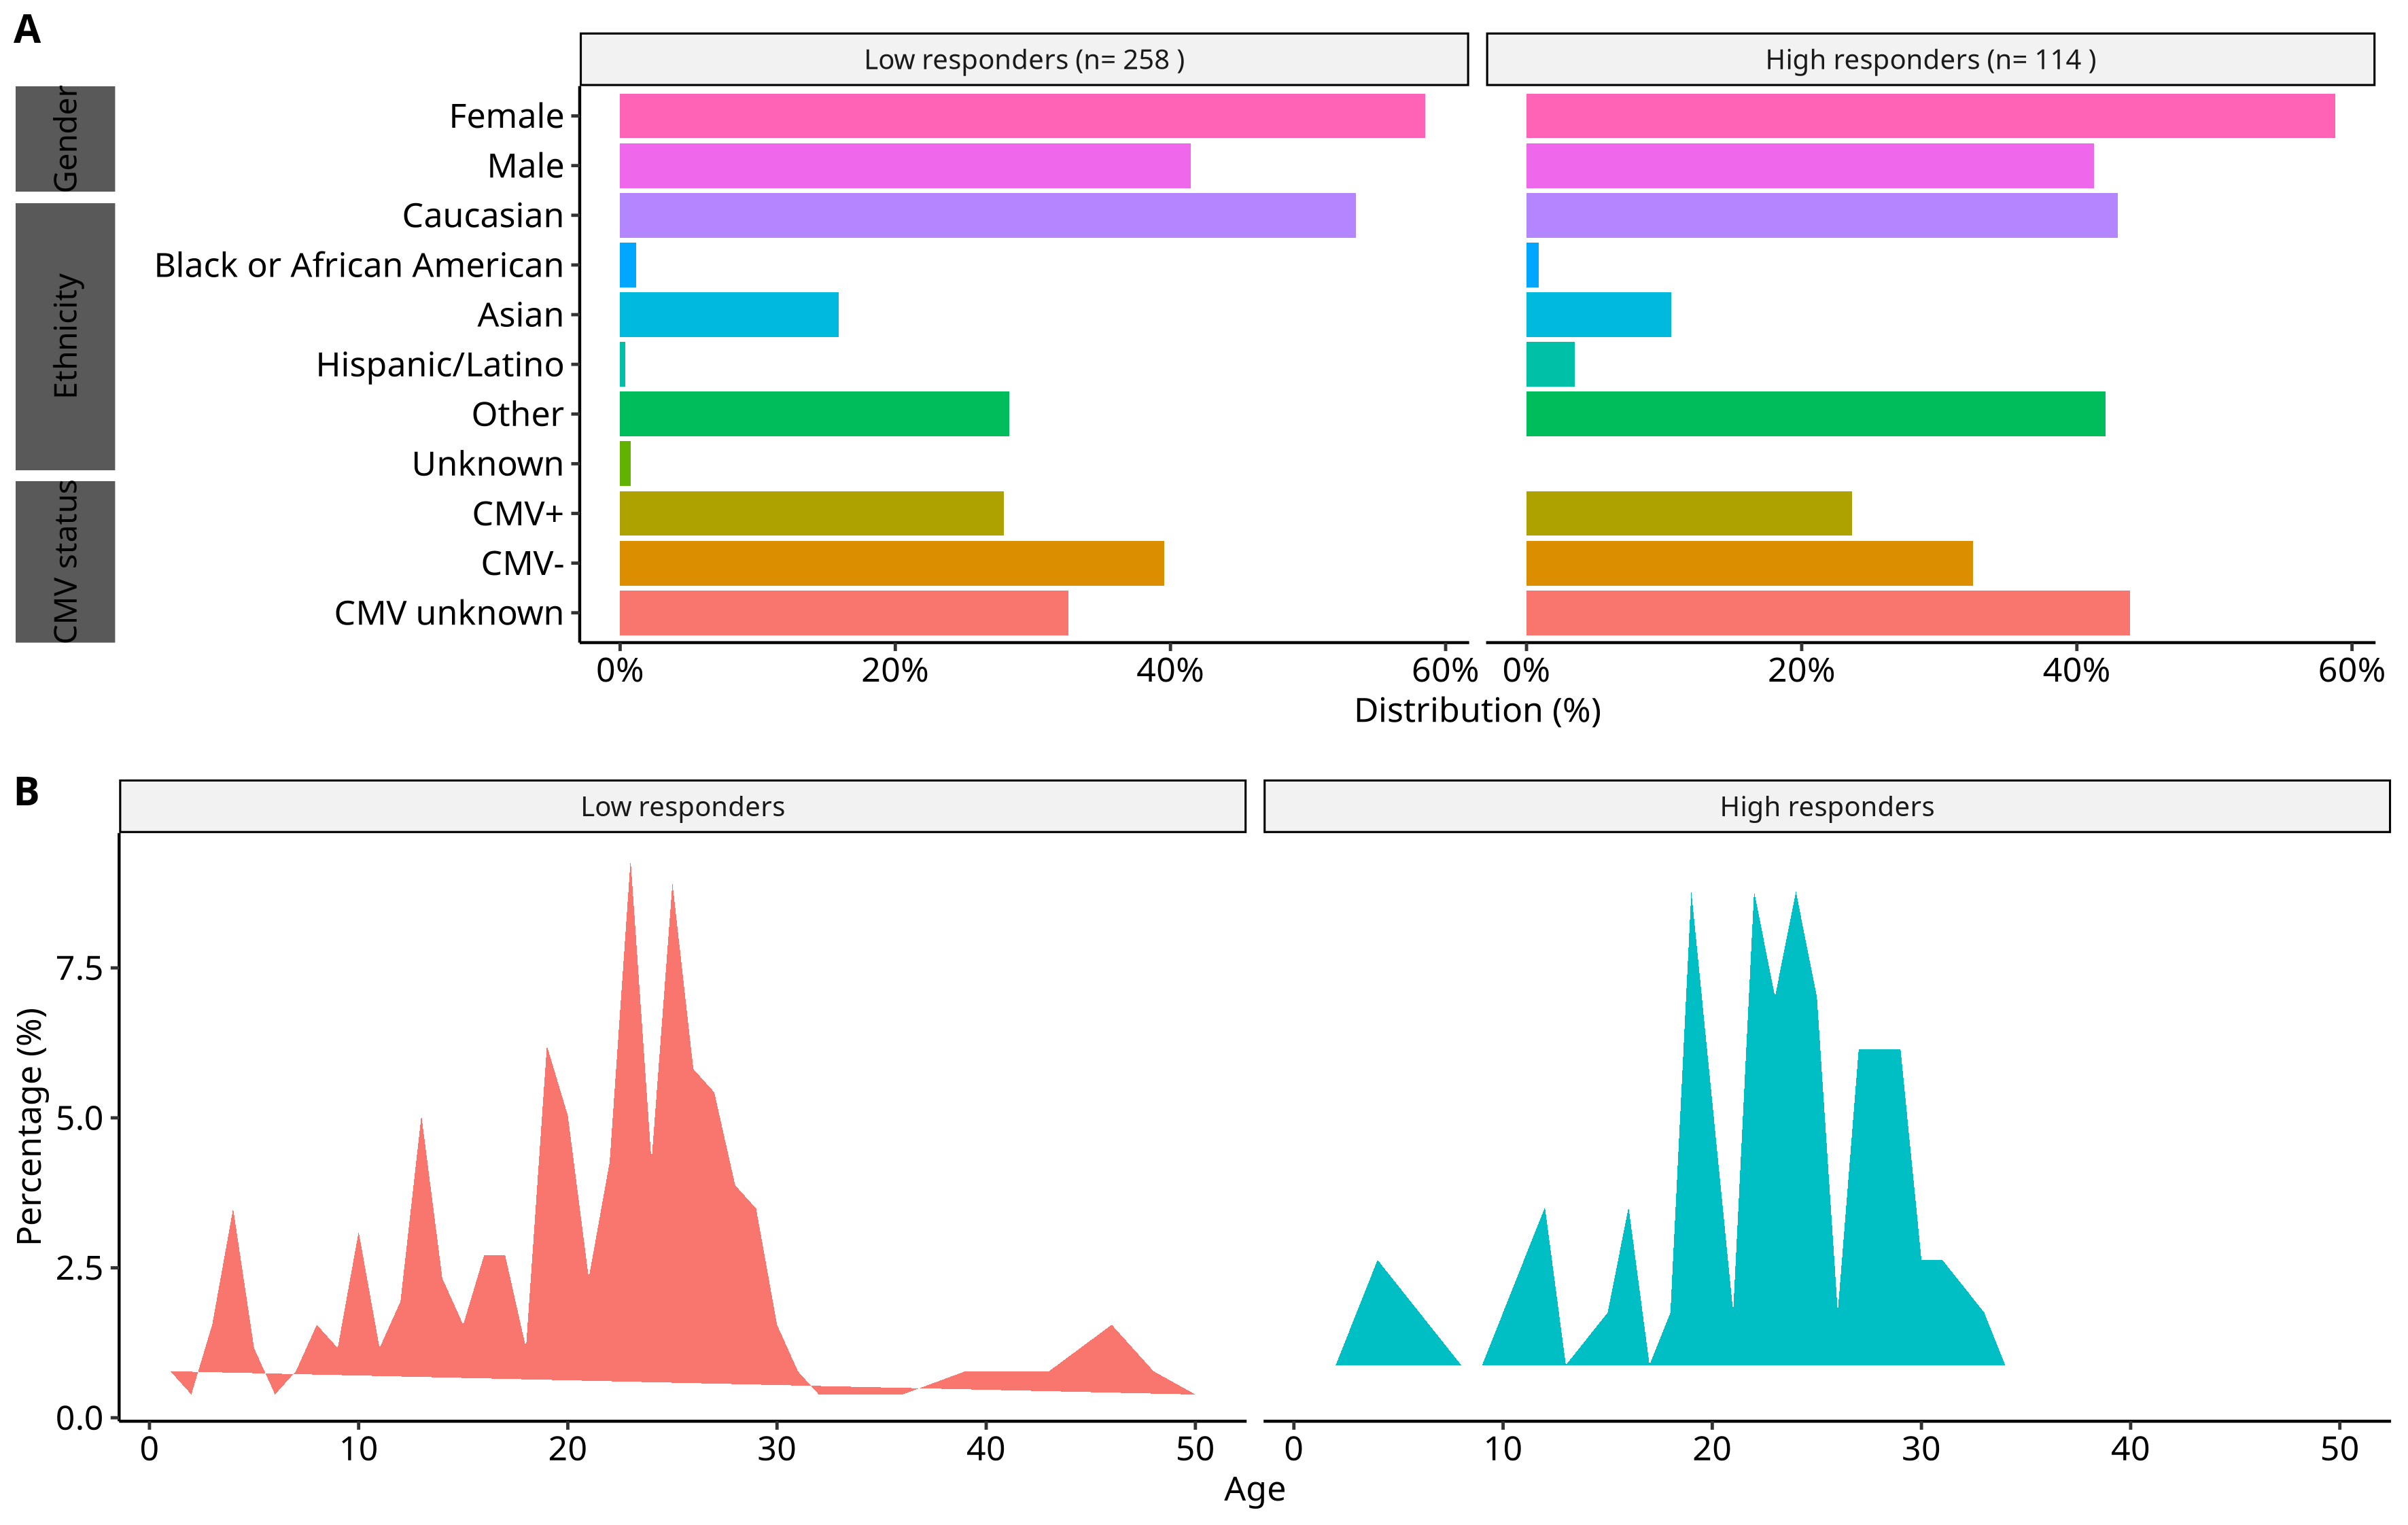
\includegraphics[width=\textwidth]{demographic}
    \caption{\textbf{A.} percentage of donors with factor property within high
    and low responder groups. Included are sex, race, and CMV status
    information. \textbf{B.} Age distribution of donors with a known response
    classification.}\label{fig:demoGraph}
\end{figure}



\begin{table}[htpb]
\centering
\begin{tabular}{ll}
\toprule
\textbf{Age (y)} & \\
\midrule
Mean $\pm$ SD & 21.02 $\pm$ 8.66\\
Median (min. to max. range) & 22.5  ( 1 - 50 )\\
\addlinespace
    \textbf{Gender} & \\
\midrule
Male (\%) & 154 ( 41.4 )\\
Female & 218  ( 58.6 )\\
\addlinespace
    \textbf{Ethnicity} & \\
\midrule
Caucasian (\%) & 187 ( 50.3 )\\
African American (Black) (\%) & 4  ( 1.1 )\\
Asian (\%) & 53  ( 14.2 )\\
Hispanic/Latino (\%) & 5  ( 1.3 )\\
Other (\%) & 121  ( 32.5 )\\
Unknown (\%) & 2  ( 0.5 )\\
\bottomrule{}
\end{tabular}
\caption{\textbf{Demographic statistics of donors with known vaccine response classification.}}\label{tbl:demoStats}
\end{table}

The data from the clinical studies consisted of 121 CSV files that were
imported into the FluPrint database. The data was used to build four tables
which will be described in the next sections, but we will not discuss technical
validation of the database construction, refer to the original work for that
\citep{tomicFluPRINTDatasetMultidimensional2019}.  The relation between the
tables is best visualised in the original work of
\citep{tomicFluPRINTDatasetMultidimensional2019}, it describes the MySql
attribute types and columns in the tables \autoref{fig:tablesFluprint}
(copied). The volume of the data is also given in the original work, per table
the number of rows and columns is reported \autoref{tbl:volumeTables}.

\begin{figure}[htpb]
    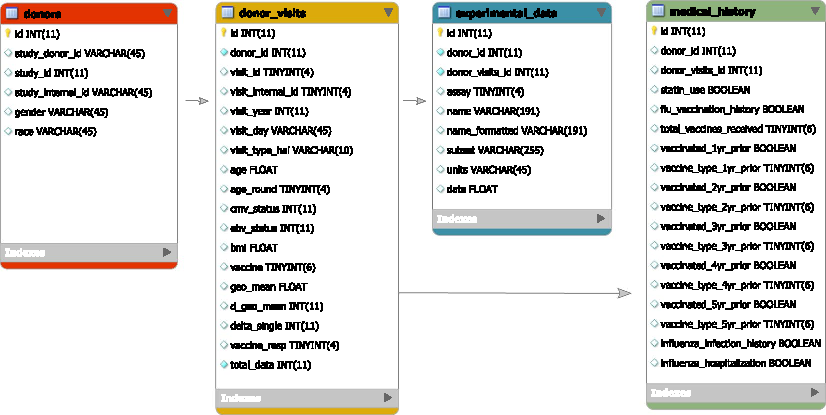
\includegraphics[width=\textwidth]{tablesFluprint}
    \caption{
        \textbf{(taken from original paper)} The FluPRINT database model. The diagram shows a schema of the FluPRINT
    database. Core tables, donors (red), donor\_visits (yellow),
    experimental\_data (blue) and medical\_history (green) are interconnected.
    Tables experimental\_data and medical\_history are connected to the core
    table donor\_visits. The data fields for each table are listed, including
    the name and the type of the data. CHAR and VARCHAR, string data as
    characters; INT, numeric data as integers; FLOAT, approximate numeric data
    values; DECIMAL, exact numeric data values; DATETIME, temporal data values;
    TINYINT, numeric data as integers (range 0–255); BOOLEAN, numeric data with
    Boolean values (zero/one). Maximal number of characters allowed in the data
    fields is denoted as number in parenthesis.
    }\label{fig:tablesFluprint}
\end{figure}

\begin{table}[htpb]
    \centering
    \begin{tabular}{lll}
        \toprule{}
        \textbf{Table name} & \textbf{Rows} & \textbf{Columns} \\
        \midrule{}
        \textit{donors} &  740 & 6 \\
        \textit{donor\_visits} & 2,937 & 18 \\
        \textit{experimental\_data} & 371,260 & 9 \\
        \textit{Medical history} & 740 & 18 \\
    \bottomrule{}
    \end{tabular}
    \caption{Volume of tables in the Fluprint database.}\label{tbl:volumeTables}
\end{table}

\subsection{Attribute types and values}

Because of the great number of attributes in the database, we discuss them by
table starting with the donors \autoref{fig:tablesFluprint}.

\subsubsection{donors table}

The \textit{donors.id} attribute is simply an enumeration of unique donors,
importantly, it is used as a key to get attributes from other tables. The
column \textit{study\_donor\_id} is an encrypted identification number. Each
donor belongs to the study identified by the \textit{study\_id}, these are the
last two digist of the name code (those starting with SLVP0 \(\cdot\cdot\)) in
the reference table \autoref{tbl:studiesDesc}, the \textit{study\_internal\_id}
is either the digit or a string containing the digit in \textit{study\_id}. The
\textit{gender} and \textit{race} attribute contain the values used in
\autoref{fig:demoGraph}, a minor note is that in the original paper "American
Indian or Alaska Native" is listed as one of the \textit{race} values but is
not used in the database. There are 5 donors whose race is "NULL", which are
mapped to unkown \autoref{fig:demoGraph}.

\begin{table}[htpb]
    \begin{tabular}{rlrlll}
\toprule{}
id & study\_donor\_id & study\_id & study\_internal\_id & gender & race\\
\midrule{}
1 & e27ad74ff9a5f2f32d8e852533f054c0 & 30 & 30 & Female & Asian\\
2 & 4a89ac4d3f4dc869e5c8e8cf862cffda & 30 & 30 & Male & Other\\
3 & a2cde6e54dec92422b0427dd49244350 & 30 & 30 & Female & Caucasian\\
4 & 0f7d8d1c13e876017ea465f99d25581f & 30 & 30 & Male & Other\\
5 & 1ed2f6409584b7b4e9720b28d794fe91 & 30 & 30 & Female & Caucasian\\
\addlinespace
6 & a575678405e9615bfb87eccfa031f7fc & 30 & 30 & Male & Other\\
\bottomrule{}
\end{tabular}
    \caption{Head of the donors table.}\label{tbl:donorsHead}
\end{table}

\subsubsection{donor\_visits table}

The donor visits table is the core table of the database, it contains donor
attributes at visit times during enrolment in clinical studies in rows that are
uniquely identified by an \textit{id} integer. Each
row also includes the \textit{donor\_id} identify the donor that visitted.

The database combines different clinical studies accross years and the data
from these studies is incomplete leading to an incomplete and hetergenous
database \autoref{tbl:visitsDesc}. For example some donors might miss their
second visit to determine their antibody levels, or the number of parameters
measured by an assay changed in the timespan of a clinical study. Unifying
these clinical studies in one database resulted in normalised but incomplete
data and heterogenous data. More specifically, every attribute in the core
table has missing value, which complicates dataset selection. One examples of
visit data of a donor is discussed to highlight important attributes and
problems in the data: that the number of visits is variable, that all columns
are incomplete, and that classification is sometimes based on single visits or
inconsistent \autoref{tbl:visit166} \autoref{tbl:visitsDesc}.

\begin{table}[htpb]
\addtolength{\leftskip} {-2cm} % increase (absolute) value if needed
\addtolength{\rightskip} {-2cm} % increase (absolute) value if needed
\begin{tabular}{lrrrrrrrrr}
\toprule{}
stat & age & cmv\_status & ebv\_status & bmi & vaccine & geo\_mean & d\_geo\_mean & vaccine\_resp & total\_data\\
\midrule{}
n & 2937.0 & 1081.0 & 548.0 & 516.0 & 2794.0 & 984.0 & 1260.0 & 1206.0 & 2937.0\\
na & 0.0 & 1856.0 & 2389.0 & 2421.0 & 143.0 & 1953.0 & 1677.0 & 1731.0 & 0.0\\
mean & 47.3 & 0.4 & 0.8 & 24.8 & 3.7 & 87.6 & 8.9 & 0.3 & 126.4\\
sd & 27.0 & 0.5 & 0.4 & 5.6 & 1.0 & 101.7 & 30.9 & 0.4 & 368.4\\
se\_mean & 0.5 & 0.0 & 0.0 & 0.2 & 0.0 & 3.2 & 0.9 & 0.0 & 6.8\\
\addlinespace
IQR & 50.2 & 1.0 & 0.0 & 6.7 & 0.0 & 105.4 & 4.0 & 1.0 & 19.0\\
skewness & 0.2 & 0.3 & -1.4 & 1.0 & -1.7 & 3.6 & 9.9 & 1.1 & 7.1\\
kurtosis & -1.5 & -1.9 & -0.1 & 2.1 & 3.0 & 26.6 & 114.9 & -0.9 & 49.7\\
\bottomrule{}
\end{tabular}
\caption{Descriptive stats of relevant numeric or binary factor columns in the
    donor visits table. For geo\_mean 0 is considered as missing data.}\label{tbl:visitsDesc}
\end{table}

Per donor all visits are enumerated in chronological order by
\textit{visit\_id} \autoref{tbl:visit166}. Further visit info includes:
\textit{visit\_internal\_id} which is a number that indicates the visit order
within an influenza season but this differs per clinical study (e.g. some use
1-2-3, orther use 0-7-28), the \textit{vist\_year} is the influenza season of
the visit, the \textit{visit\_day} is the number of days relative to the date
of vaccination,  \textit{age} and \textit{age\_round} indicate the donor's age
at time of the visit, and \textit{bmi} gives the donor bmi at visit time, and
lastly \textit{visit\_type\_hai} is the intent of the visit which is either
"pre", "post", or "other",

During the "pre" visit a virological assay is performed to determine the CMV
and Epstein-Barr virus (EBV) status of the donor, which are indicated by the
binary variables \textit{cmv\_status} and \textit{ebv\_status}.

To measure vaccine response to a vaccine which is indicated by an id
\autoref{tbl:remapVaccine} in \textit{vaccine}, the hemagglutination inhibition
assay (HAI assay) is used. The procedure measures the influenza antibody titers
before vaccination during the \textit{visit\_type\_hai} "pre" visit of a
participant, and 28 days after vaccination during a "post" visit. The geometric
mean titer (GMT) at each visit is calculated, and a fold change in GMT is
calculated as the ratio of the GMT at day 28 (post) and during the first visit
(pre). These values are \textit{geo\_mean} and \textit{d\_geo\_mean},
\textit{d\_single} is the antibody titer fold-change per strain of virus used
in the vaccine, it is unclear how this value is aggregated over different
strains and is left out of further analysis.  This data was used to classify
donors in high or low responders according to FDA guidelines \cite{},
individuals are high-responders if they seroconverted (4-fold or greater rise
in HAI titer) and were seroprotected (GMT HAI \(\ge\) 40) after vaccination.
The seasonal vaccine response classifications are given by the binary variable
\textit{vaccine\_resp}.

The assays performed to get a serological/immunlogical profile of the donor
before vaccination are described later in the section of the experimental data
table, all assays are listed in the original work
\cite{tomicFluPRINTDatasetMultidimensional2019} and are summarised here
\autoref{tbl:assays}, the total rows of assay data is given by
\textit{total\_data}.

\begin{table}[htpb]
\addtolength{\leftskip} {-2cm} % increase (absolute) value if needed
\addtolength{\rightskip} {-2cm} % increase (absolute) value if needed
\begin{tabular}{rrrlrrrlrrrrr}
\toprule{}
visit\_id & year & day & type & age & cmv & ebv & bmi & vaccine & geo\_mean & d\_geo\_mean & response & assay\_data\_rows\\
\midrule{}
1 & 2011 & 0 & pre & 20 & 1 & 1 & 30.31 & 4 & 25.20 & 6 & 0 & 343\\
2 & 2011 & 7 & other & 20 & 1 & 1 & NULL & 4 & 0.00 & 6 & 0 & 51\\
3 & 2011 & 28 & post & 20 & 1 & 1 & NULL & 4 & 160.00 & 6 & 0 & 51\\
4 & 2012 & 0 & pre & 21 & 1 & 1 & 30.31 & 4 & 9.28 & 4 & 0 & 292\\
6 & 2013 & 0 & pre & 22 & 1 & 1 & 30.31 & 4 & 15.91 & 2 & 0 & 2877\\
\addlinespace
7 & 2013 & 7 & other & 22 & 1 & 1 & NULL & 4 & 0.00 & 2 & 0 & 63\\
8 & 2013 & 28 & post & 22 & 1 & 1 & NULL & 4 & 26.75 & 2 & 0 & 82\\
\bottomrule{}
\end{tabular}
\caption{Visit data of donor 166 from study SLVP021 \autoref{tbl:studiesDesc},
where participants are only vaccinated once.
Number of visits and data collected at visit varies, classification is
inconsistent with \( \geq 40\) and 4-fold increase
rule in 2011.}\label{tbl:visit166}
\end{table}

The most important data related to the visits of donor 166 is shown in Table
\ref{tbl:visit166}.  The vaccine response classification is calculated based on
the GMT in the "pre" and "post" visits.  This classification is done per
influenza season, but the HAI assay requires a "pre" visit and a "post" visit
28 days later to measure the difference in GMT.  However, sometimes a
classification is given when there is only one visit record in a season, like
in 2012 for donor 166 \autoref{tbl:visit166}.

\begin{figure}[htpb]
    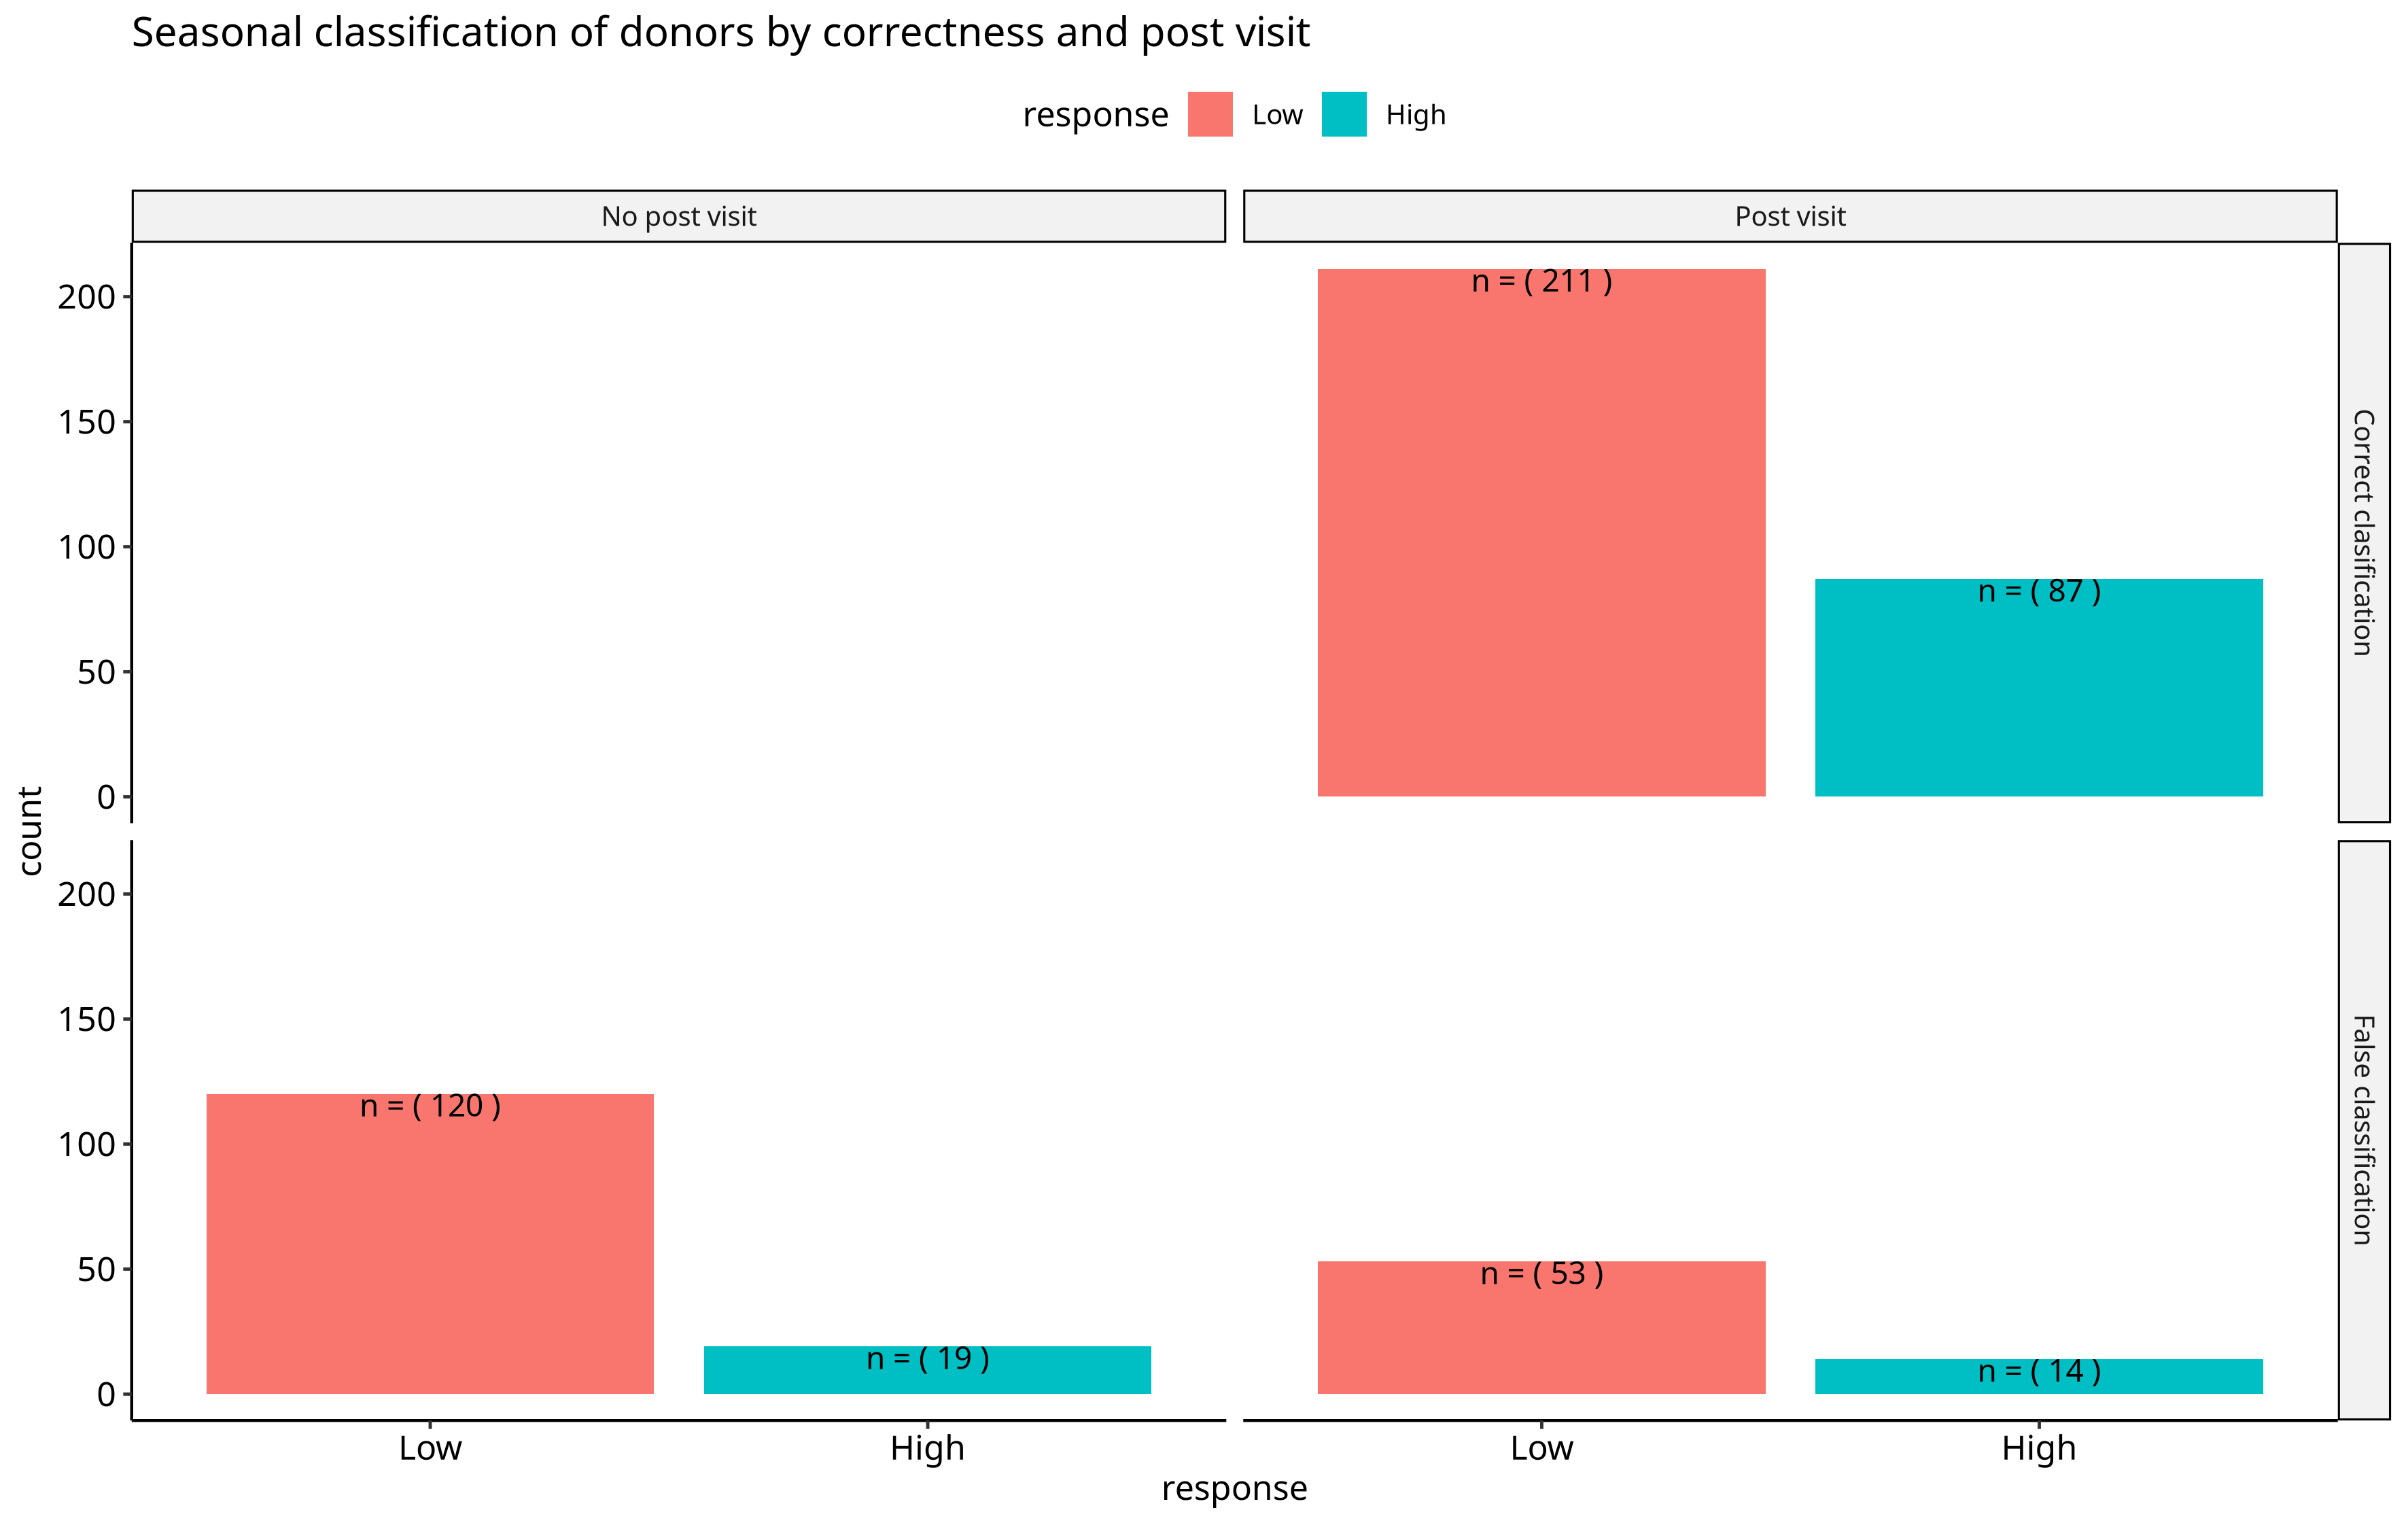
\includegraphics[width=\textwidth]{season_classification}
    \caption{}\label{fig:classInconsistent}
\end{figure}

The example of donor 166 contains an inconsistency in the classification, in
2011 the GMT \textit{geo\_mean} increases from 25.20 to 160.00, and the
\textit{d\_geo\_mean} is 6, but in this season the donor is wrongly classified
as a low responder \autoref{tbl:visit166}. Because of this the seasonal
classification of donors was investigated using the seroprotection and
seroconversion criteria \ref{fig:seasonalClasses}, records of incorrectly
labelled donors are also saved as a spreadsheet. This data is inconsistent in
the database, but the most likely explanation is that antibody titer for one
strain of virus did not meet the high response classification criteria. In this
work it is considered as inconsistent because individual strain titer data is
not in the database, but classification is therefore not necessarily incorrect.
Hence the classification will be used in this work without further selection.

\subsubsection{Experimental data table}

\begin{table}[htpb]
    \begin{tabularx}{\textwidth}{Xp{0.5\textwidth}X}
\toprule{}
        \textbf{Name} & \textbf{Description} & \textbf{id} (\textit{experimental\_data.assay})\\
\midrule{}
        (Multiplex) cytokine assays & Multiplex ELISA using Luminex polysterene
        bead or magnetic bead kits. Measures serum cytokine/hormone level in
        z.log2 units using fluorescent antibodies. & 3, 6, 15, 16\\
        \addlinespace
        Flow and mass cytometry assays & uses labeled antibodies to detect antigens on
        a cell surface to identify a subset of a cell population, units are in
        percentage of parent population. & 4, 9, 13, 17 \\
        \addlinespace
        Phosphorylation cytometry assays & Uses antibodies to measure
        phosphorylation of specific proteins stimulated by an immune system event
        belonging to cell population subsets. Units are a fold change between
        stimulated and un-stimulated cells, for mass cytometry arcsin readout difference,
        fold-change of 90th percentile readout values otherwise.  & 7, 10 (mass cytometry) (flow cytometry)\\
        \addlinespace
        complete blood count (CBCD) & Different cells are counted using flow
        cytometry Units are usually in Count/$\mu$L & 11 \\
        \addlinespace
        meso scale discovery assays (MSD) & A setup where serum cytokines or hormones
        are captured with antibodies, and then detected by using a detection
        antibody. Units are arbitrary intensity & 2, 12, 14 \\
\bottomrule{}
\end{tabularx}
    \caption{assays table}\label{tbl:assays}
\end{table}


Assays performed in visits are remapped, but the values in the
database do not correspond to the reported table \autoref{tbl:remapVaccine}.
Actual assay type, data units, and id in the database are reported here
\autoref{tbl:assays}.

\fpfig{exp_data_numbers}{.7}
{Feature count per individual assay id, assay type, stratisfied in either response status or study}
{caption}
{fig:featureNumbers}

In total there are data from 14 different assays, not counting the virological
and HAI antibody assays \autoref{tbl:assays}. The virological assays include
the cmv virus status and ebv status, and is not used in this work because it is
done in a smaller subset of studies. Those 14 assays have been aggregated in
this work to 5 different types of experiments: the multiplex assays measure
serum molecules such as cytokines and other signaling molecules, flow and mass
cell cytometry measure the phenotype of specific immune related cells,
phosphorylation flow and mass cytometry measures the phosphorylation signaling
pathway activation after an immune stimulation, the blood count measures the
count of cells in the blood, and meso scale discovery (MSD) measures hormones
or cytokines from the blood.

\begin{figure}[htpb]
    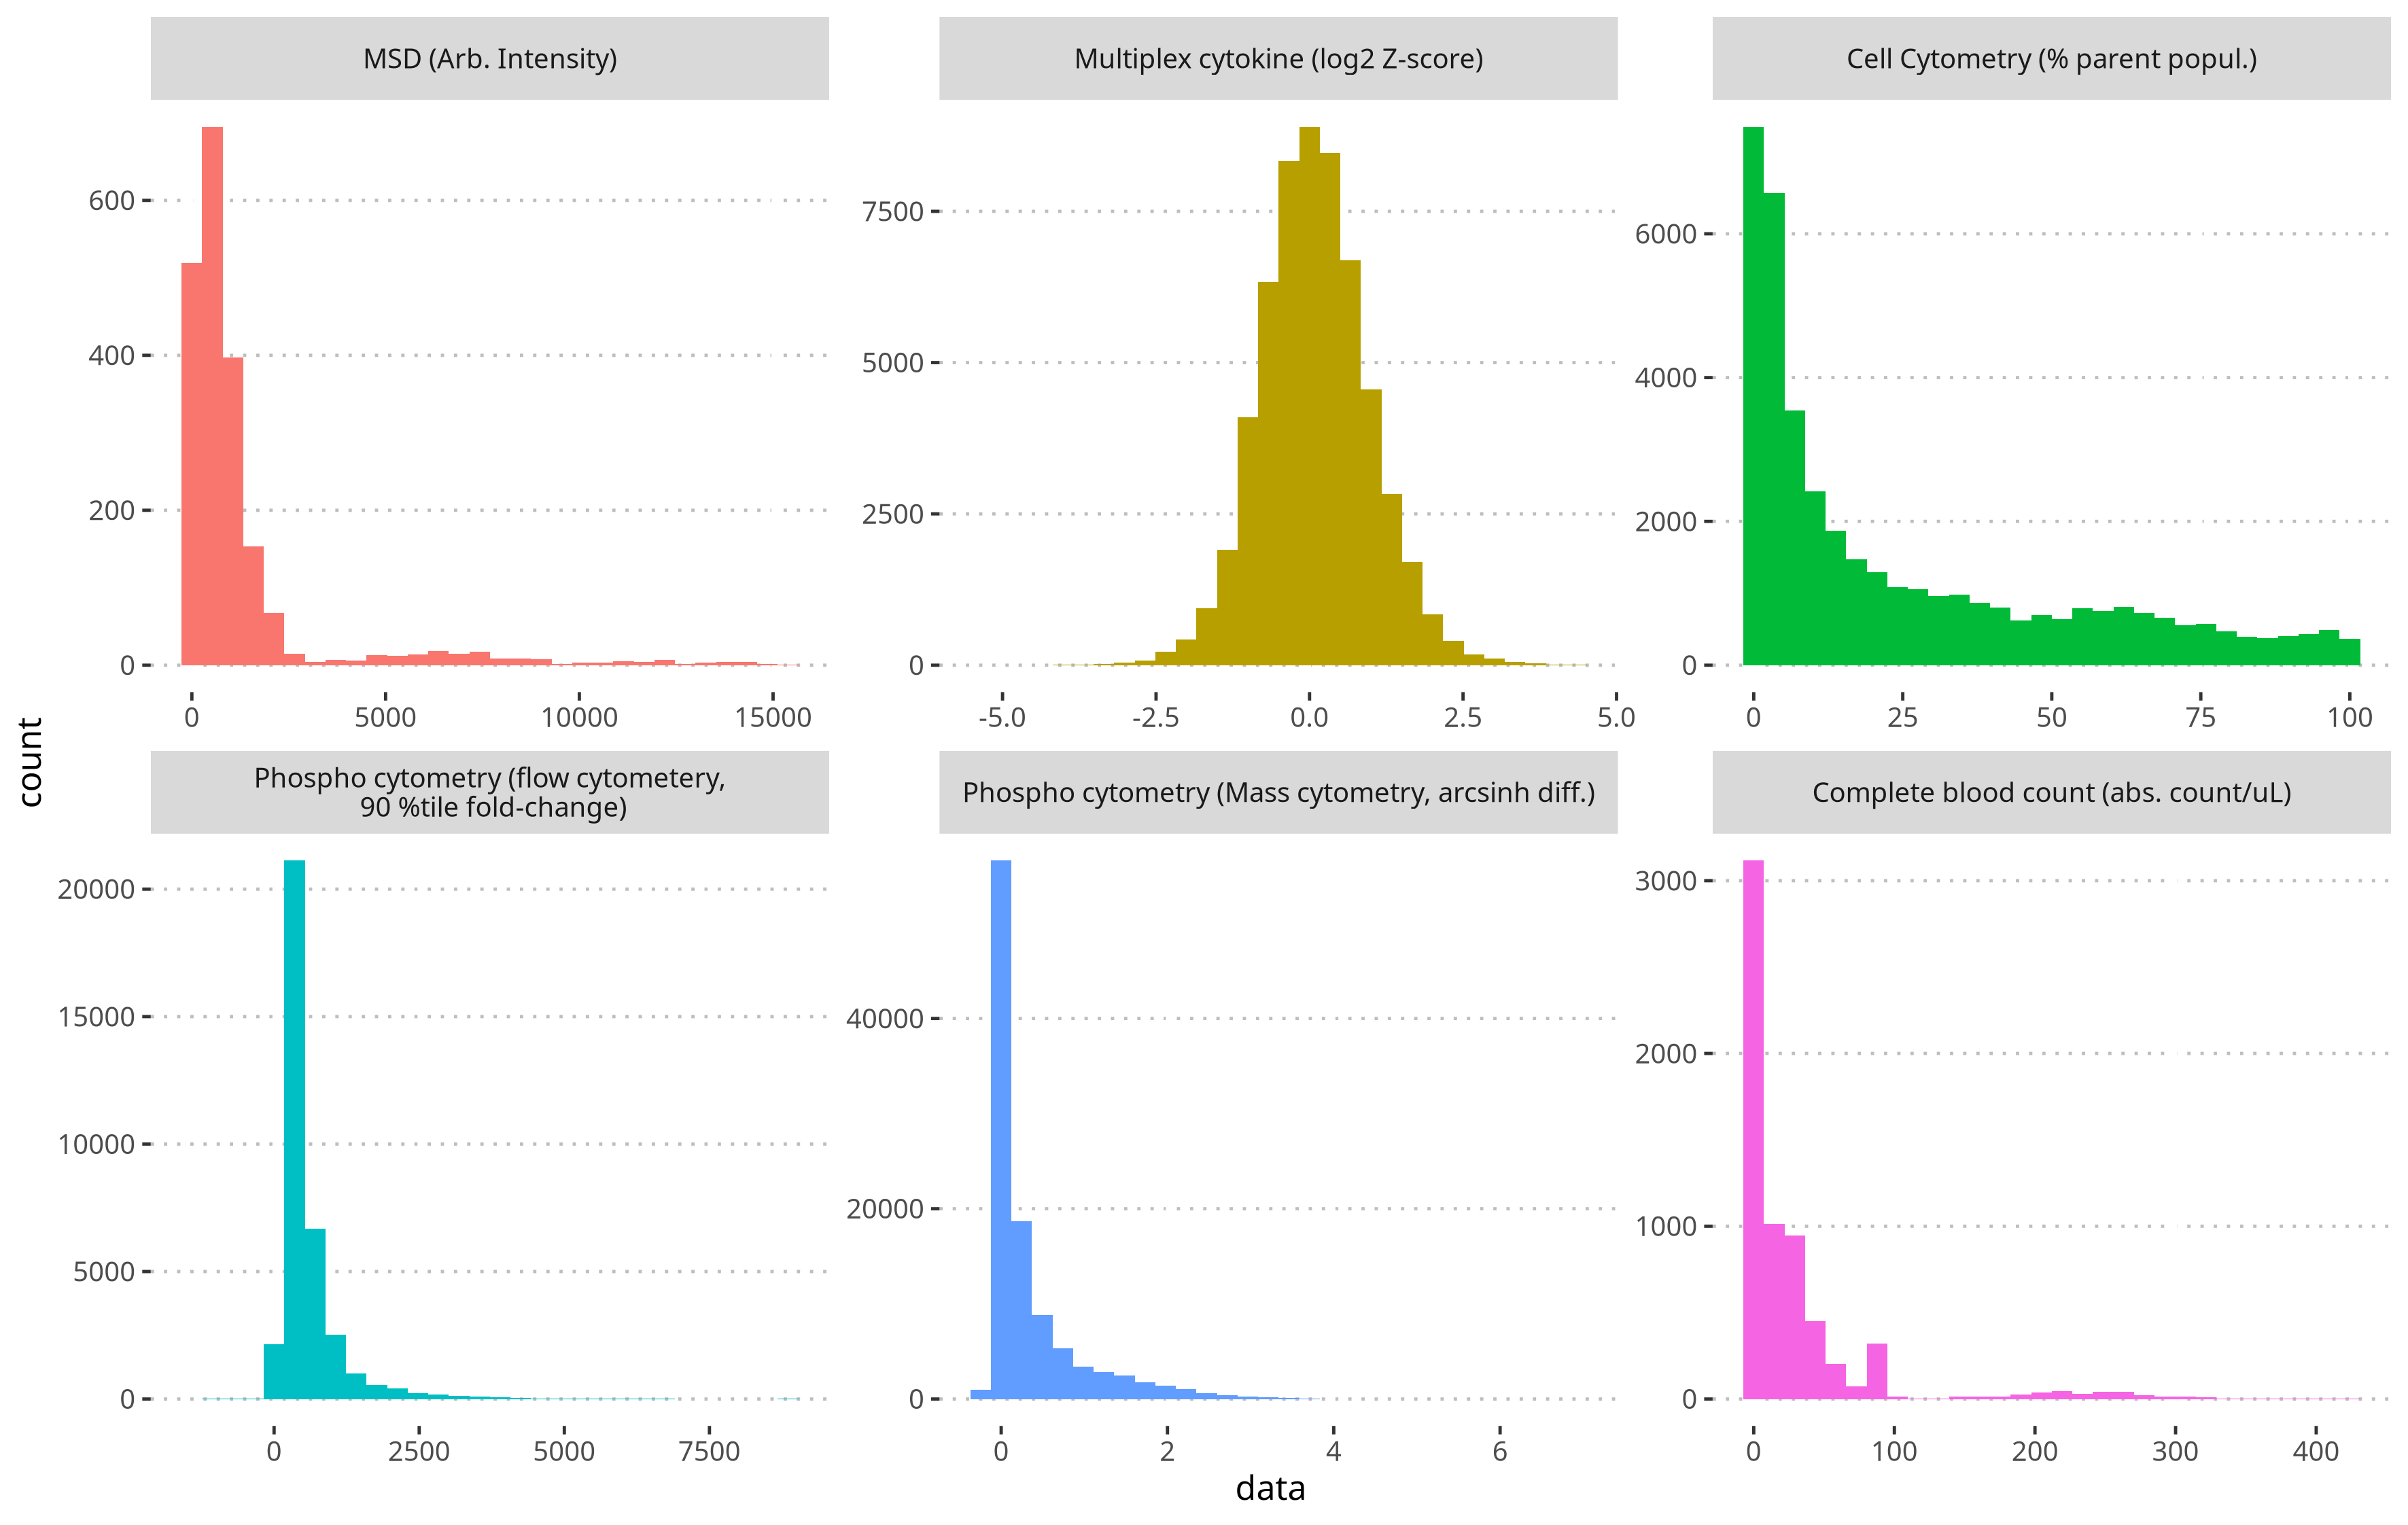
\includegraphics[width=\textwidth]{assay_value_distributions}
    \caption{noise in 90th \%tile}\label{fig:assayDistr}
\end{figure}

The experimental data table contains all features recorded for a donor visit.
The number of features collected for each visit is large and varies greatly
(mean at 126 , \(\pm \)368 SD) \autoref{tbl:visitsDesc}, and in total there are
3285 different features measured across all clinical studies. However, not
every assay is done in every clinical study \autoref{fig:featureNumbers} and
over the years the data generated by assays has changed, so a table with all
features as columns and all donors as rows would be extremely sparse (and
crashes R due to RAM limitations).  Describing the 3285 different features in
this sparse table would be impossible, but assay value distributions across
studies are shown to follow normal or power distributions
\autoref{fig:assayDistr}. The features included 102 blood-derived immune cell
subsets analyzed by mass cytometry. It also included the signaling capacity of
over 30 immune cells subsets stimulated with seven conditions, which were
evaluated by measuring the phosphorylation of nine proteins. Additionally, up
to 50 serum analytes were evaluated using Luminex bead arrays
\citep{tomicSIMONAutomatedMachine2019}.

No correlation analysis was done, since this is complicated by the great number
of features and sparseness in the data.

\begin{figure}[htpb]
    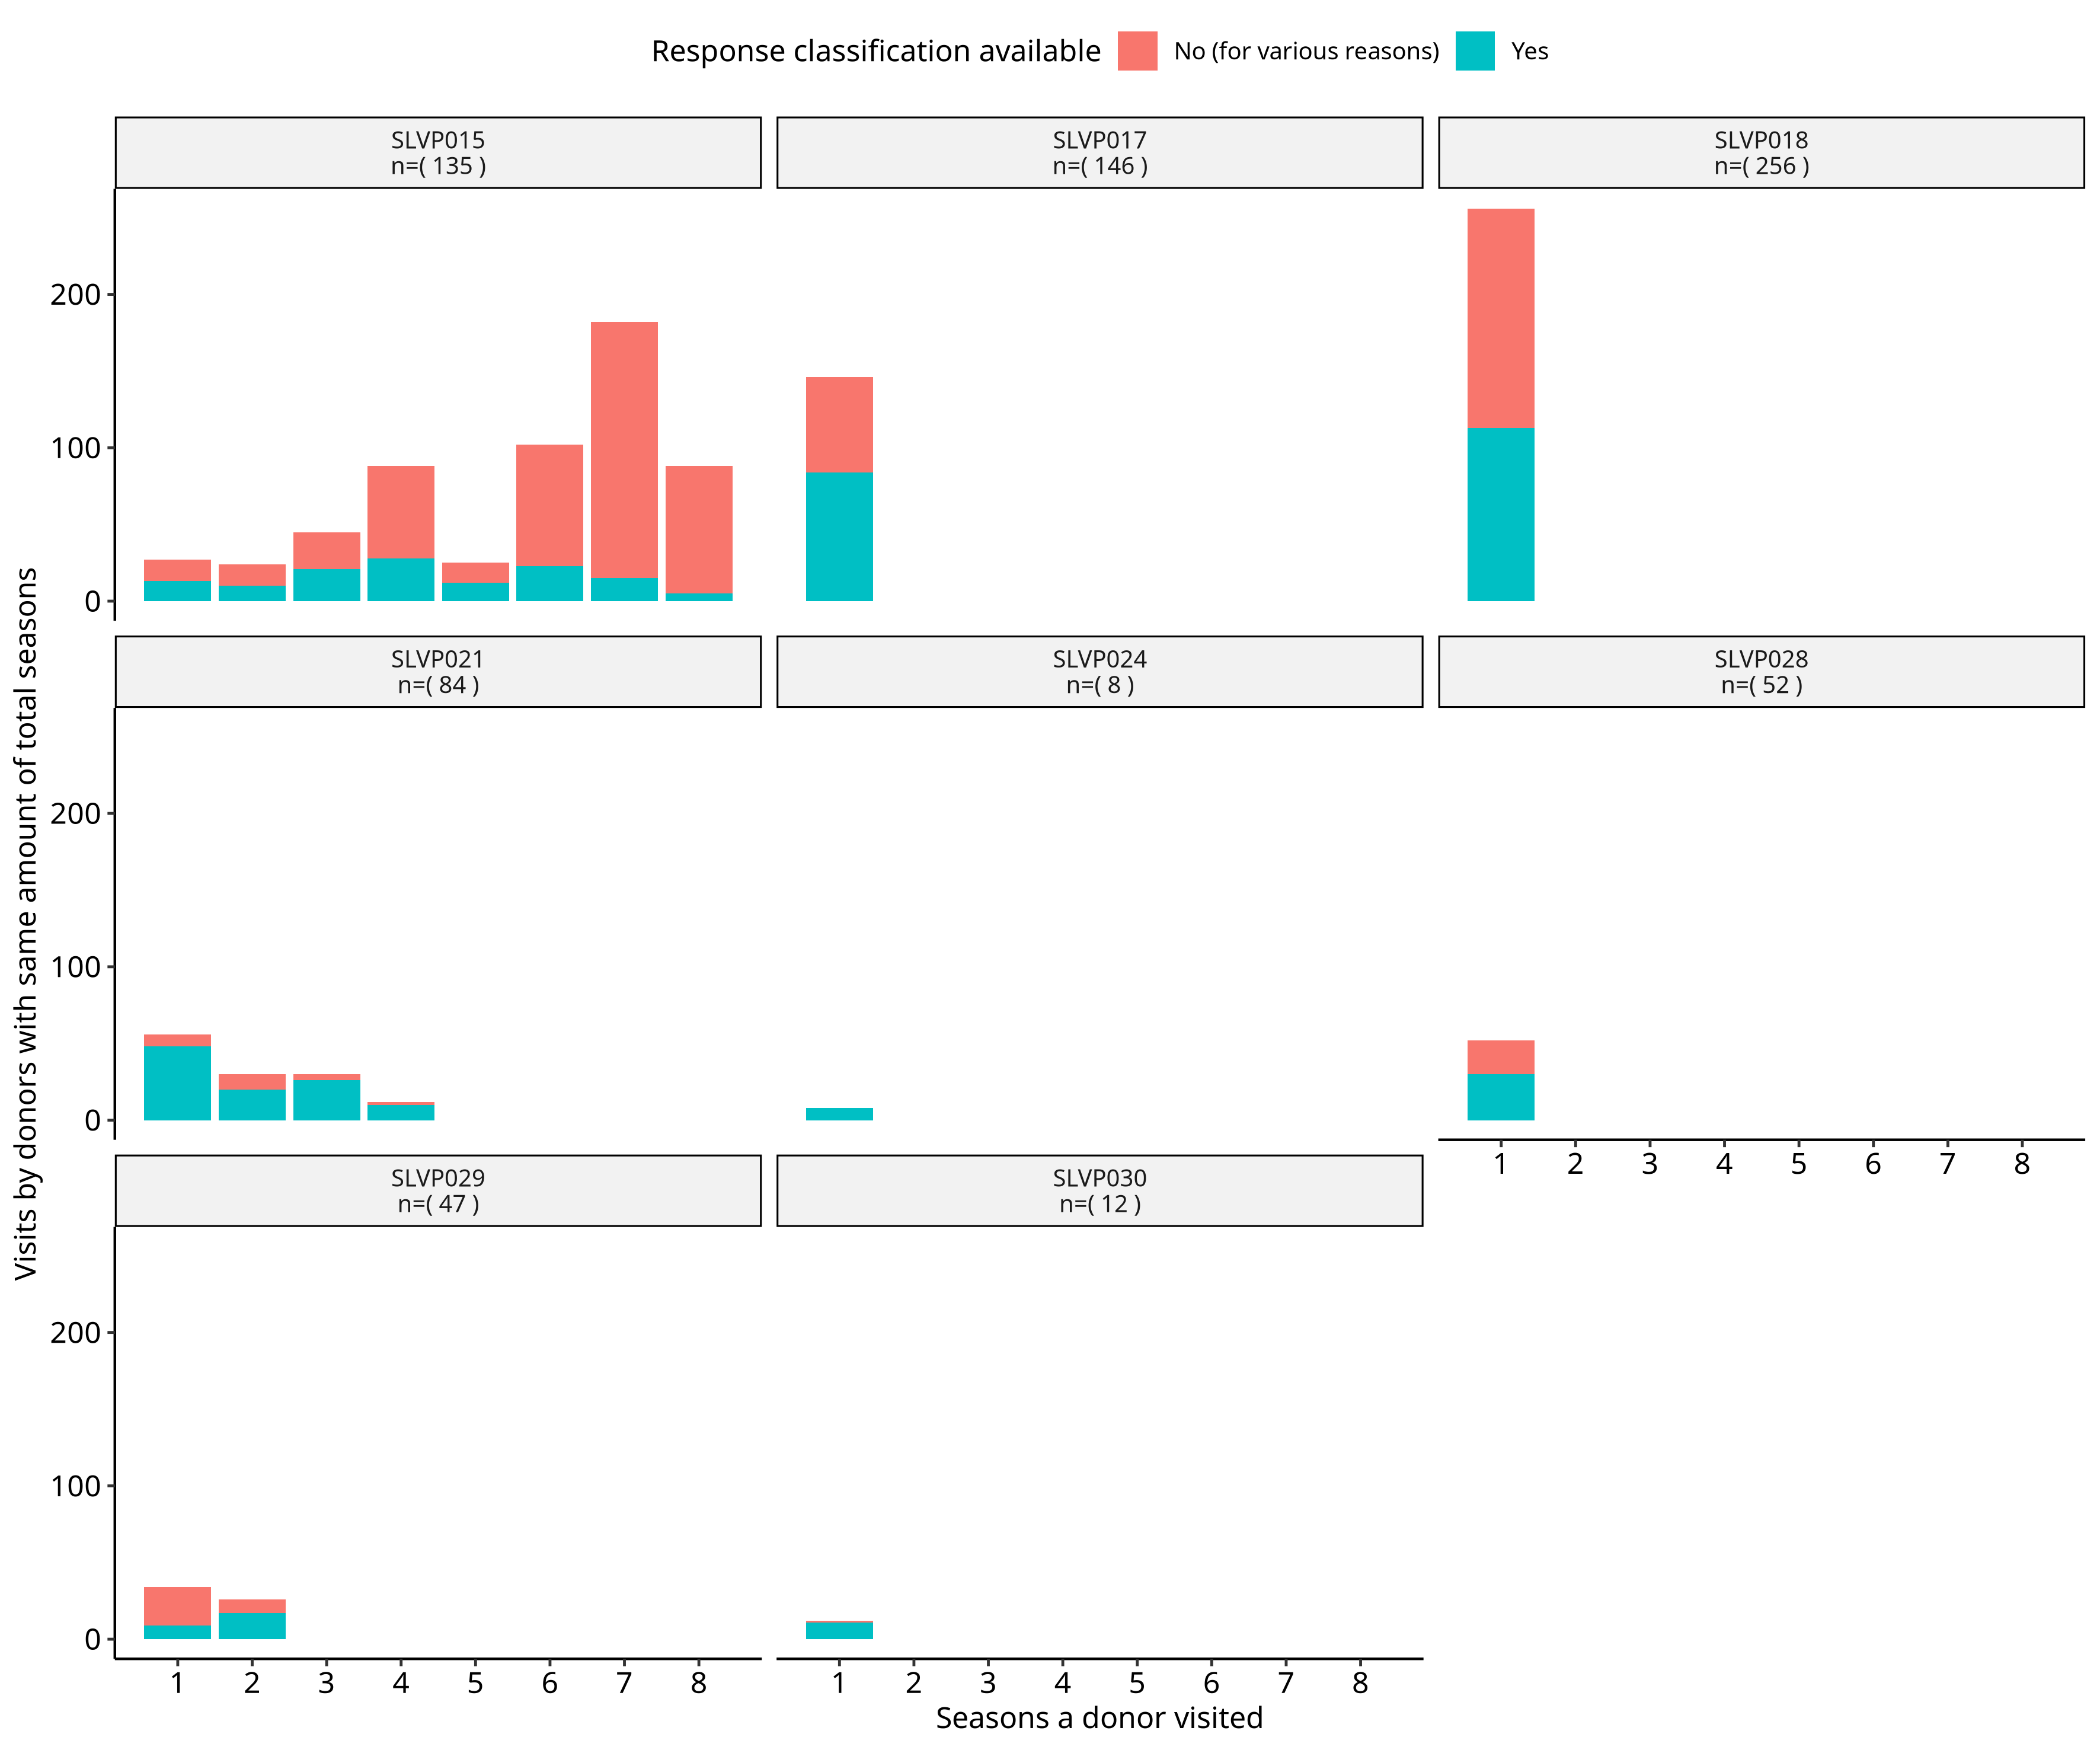
\includegraphics[width=\textwidth]{repeat_visits_per_study}
    \caption{the number of donors that visited per number of influenza seasons
    they visited (years), per study. The color indicates the number of visits for which a
    classification was available, counted within the groups of donors that
    visited the same amount of times.}\label{fig:repeatVisits}
\end{figure}

What further complicates selecting data is repeat visits of donors, and missing
visits. The problem of repeat visits over a span of multiple influenza seasons
is that not the same assay types are done, and that repeat visits are only a
small portion of the database. The data is also not suitable right away for
studying the effect of repeat vaccination on high versus low vaccine reponse,
since the classification in the longitudal study (SLVP015) is mostly not
available \autoref{fig:repeatVisits}.

For example exploring the effect repeat vaccination has an response rate would
first require manual labelling of high and low responses, at least for the
cases where it is possible based on the GMT data. Those cases are when
classification is set to a null value even though GMT data is available.  The
reason for this null value assignment is reported, but the pattern seems to set
the vaccine response to null if there is not enough assay data measured.

\subsection{Data quality}

The database has issues that are inherent to combining multiple studies and the
classification is inconsistent in some cases \autoref{fig:classInconsistent},
or often missing completely because no HAI antibody assay data was available or
the classification was set to a null value by the database authors because
possibly the antibody titer for a single strain of virus in the vaccine was too
low (this data is not in the database) \autoref{fig:repeatVisits}.  The main value of
the database is the assay data that is fully represented in all studies and
across all years, but this information is hard to access since all studies do
not use overlapping assays \autoref{fig:featureNumbers}, resulting in high
sparsity data. Further, the sample size that can be used for further studies is
limitted, since the high versus low vaccine response is only available for a
small subset of the data.

Specific attributes that have great amounts of missing values are the
virological and HAI assay data, the last is used for the vaccine response
classifcation. Potential for Studying the correlation of these values with
vaccine response is thus limitted. Nevertheless assay data is often available
and could be used to identify immunological factors that correlate with other
data, such as repeat vaccination, the exploration of this effect is outside the
scope of this work due to the data sparsity issues.

\section{Data preparation}

\subsection{Data selection}

The data selection used in this work is based the query used in \spaper
\autoref{lst:QueryTemplate}. Using this query generates a subset of \flup
comprised data from 5 clinical studies, most importantly the longitudal study
SLVP015 \autoref{tbl:studiesDesc}. Presumably, the authors of \spaper included
only the first visit of donors because the classification is the most complete
in this dataset \autoref{fig:dataRepeatvisits}. In this work we use this query
to generate initial first visit datasets. However, to explore repeat vaccination,
we select a subset of this data that includes donors with a repeat visit in a
second influenza season.

\begin{figure}[htpb]
    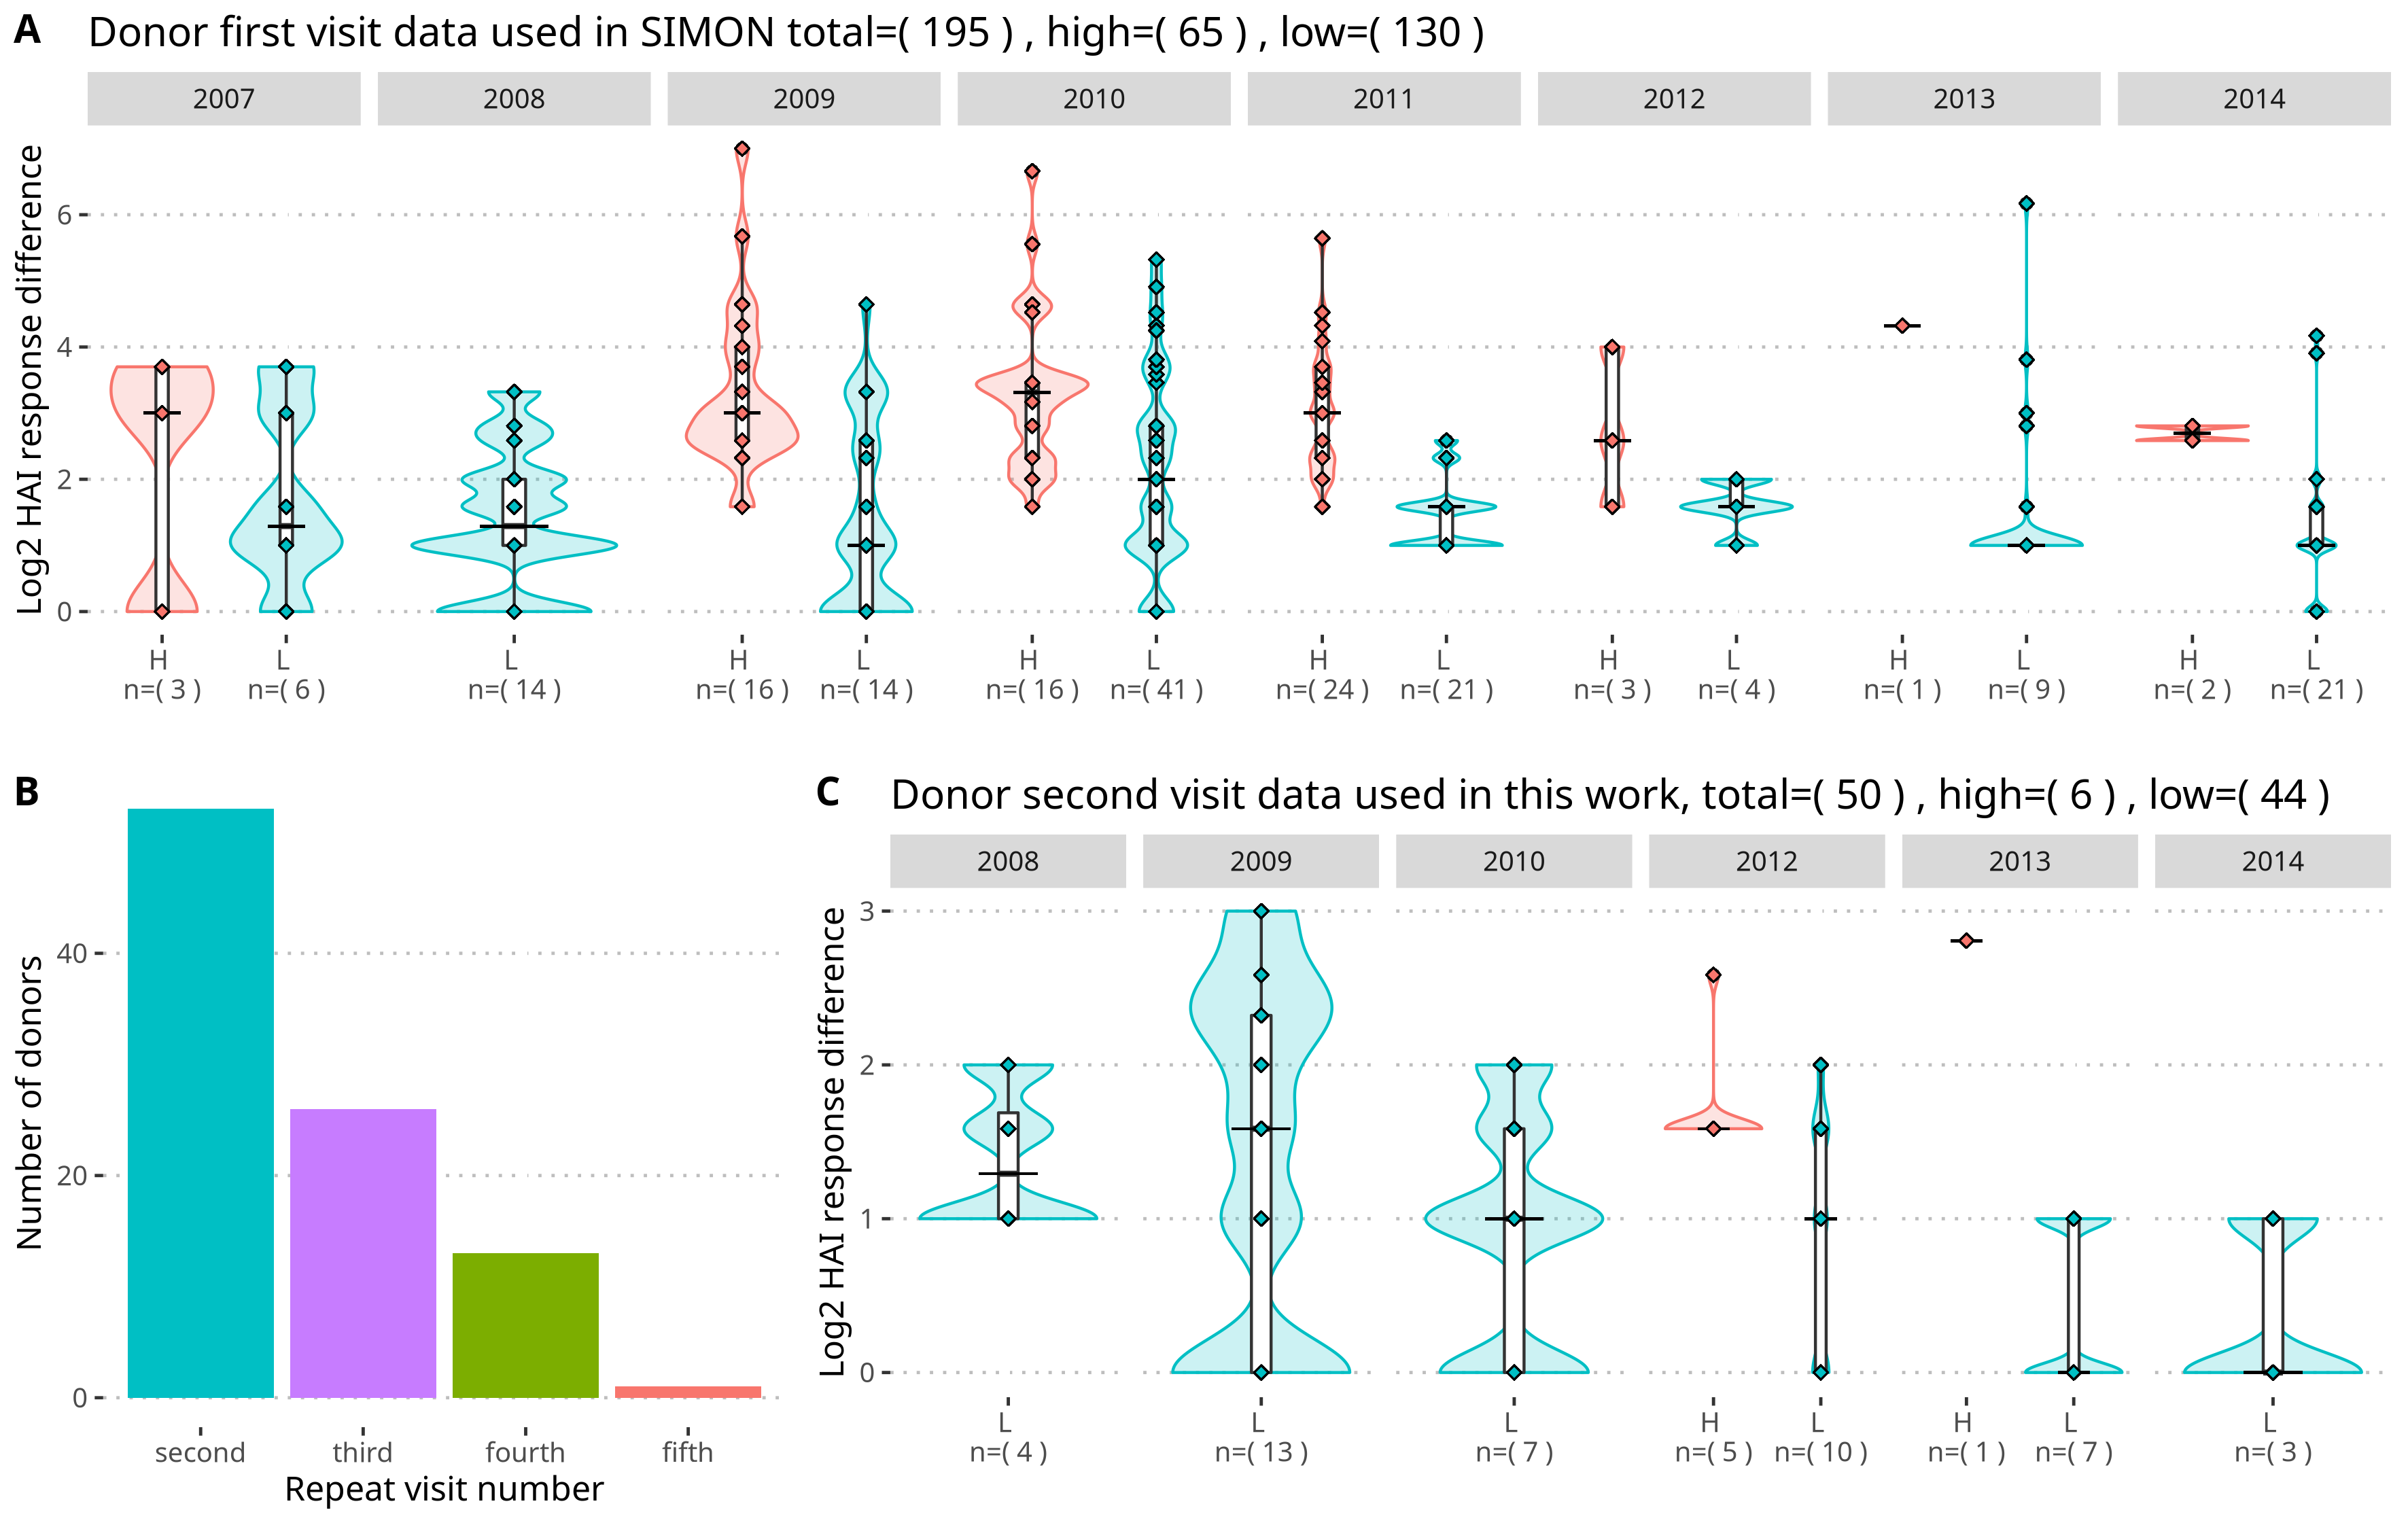
\includegraphics[width=\textwidth]{data_selection}
    \caption{caption}\label{fig:dataRepeatvisits}
\end{figure}

The initial query used in \spaper generated a long table for in total 3285
different features recorded at the first visit of 195 donors in different
studies and years (referred to as \firstvis). The observable pattern in this
data is that low responding donors are overrepresented and that the
classification is consistent with the log2 \gmt change
\autorefsub{fig:repeatVisits}{A}. Unfortunately, the number of donors in the
\firstvis that returned in other influenza seasons  decreases quickly, limiting
possibilities of comparing models built on \firstvis and subsequent visit data
\autorefsub{fig:repeatVisits}{B}. Nevertheless, we selected the \secondvis to
explore repeat vaccinations. The \secondvis has an exacerbated class imbalance
that precludes training any models, therefore we use the \secondvis to explore the
knowledge gained by models trained on the \firstvis
\autorefsub{fig:repeatVisits}{C}.

\begin{minipage}{\linewidth}

\begin{lstlisting}[caption=Applying the mulset algorithm and preparing the data, label={lst:mulsetStep}]
generate intersection datasets suitable for analysis
for {each donor in data} do:
    Calculate intersection between donor and all other donors using mulset algorithm
    Skip sets that have less than 5 features and less than 15 donors in common
end for;

for {each set in generated datasets} do:
    Partition data in training (75\%) and test (25\%) split
    Skip sets that have less than 10 donors in the test set
end for;

for {each set in prepared datasets} do:
    calculate number of donors that visited a second influenza season
    skip dataset if it is not in the top3 of datasets containing the highest number of second visitors
end for;
\end{lstlisting}
\end{minipage}

The \firstvis had a total of 640575 cells of which 596736 values were
missing (sparsity of 93\%) because of the heterogeneity in clinical studies and
years where data was collected. In \spaper missing data is not imputed because
there is not enough prior knowledge. And, since every donor had a missing
feature, dropping all rows/donors was not an option either. A solution used in
\spaper was generating complete tables comprising subsets of donors that had
all features in common using the mulset algorithm \autoref{lst:mulsetStep}
\autoref{fig:mulsetAlg}.

In this work the procedure in \spaper was replicated and extended to generate
usable datasets \autoref{lst:mulsetStep}. Firstly, there were duplicate
measurements of features in the \firstvis, these were aggregated to unique
feature records using the mean.  Second, the mulset R package was used to
generate 47 complete datasets. These datasets were then reduced to 36 by
selecting those that had at least 5 features and 15 donors. Finally, the
datasets were split into train (75\%) and test (25\%) sets, and datasets with
less than 10 donors in the test set were discarded reducing the number of
datasets to 20 \autoref{tbl:mulsetDatasets}.

\begin{table}[htpb]
    \begin{tabularx}{\textwidth}{XXXXX}
\toprule{}
        dataset & Rows x Cols (Donors x Features) & total (low / high (low \%)) & train (low / high) & test (low / high)\\
\midrule{}
1 & 61 x 78 & 43 / 18 ( 0.7 ) & 33 / 14 & 10 / 4\\
2 & 105 x 101 & 62 / 43 ( 0.59 ) & 47 / 33 & 15 / 10\\
3 & 140 x 50 & 94 / 46 ( 0.67 ) & 71 / 35 & 23 / 11\\
4 & 63 x 269 & 38 / 25 ( 0.6 ) & 29 / 19 & 9 / 6\\
5 & 62 x 293 & 38 / 24 ( 0.61 ) & 29 / 18 & 9 / 6\\
\addlinespace
6 & 68 x 237 & 42 / 26 ( 0.62 ) & 32 / 20 & 10 / 6\\
7 & 67 x 44 & 47 / 20 ( 0.7 ) & 36 / 15 & 11 / 5\\
8 & 111 x 93 & 66 / 45 ( 0.59 ) & 50 / 34 & 16 / 11\\
9 & 73 x 54 & 58 / 15 ( 0.79 ) & 44 / 12 & 14 / 3\\
10 & 40 x 105 & 28 / 12 ( 0.7 ) & 21 / 9 & 7 / 3\\
\addlinespace
11 & 46 x 97 & 32 / 14 ( 0.7 ) & 24 / 11 & 8 / 3\\
12 & 137 x 53 & 78 / 59 ( 0.57 ) & 59 / 45 & 19 / 14\\
13 & 48 x 42 & 35 / 13 ( 0.73 ) & 27 / 10 & 8 / 3\\
\textbf{14} & \textbf{91 x 38} & \textbf{62 / 29 ( 0.68 )} & \textbf{47 / 22} & \textbf{15 / 7}\\
15 & 42 x 37 & 36 / 6 ( 0.86 ) & 27 / 5 & 9 / 1\\
\addlinespace
\textbf{16} & \textbf{92 x 26} & \textbf{62 / 30 ( 0.67 )} & \textbf{47 / 23} & \textbf{15 / 7}\\
17 & 88 x 6 & 68 / 20 ( 0.77 ) & 51 / 15 & 17 / 5\\
18 & 82 x 87 & 56 / 26 ( 0.68 ) & 42 / 20 & 14 / 6\\
\textbf{19} & \textbf{151 x 51} & \textbf{92 / 59 ( 0.61 )} & \textbf{69 / 45} & \textbf{23 / 14}\\
20 & 83 x 75 & 56 / 27 ( 0.67 ) & 42 / 21 & 14 / 6\\
\bottomrule{}
\end{tabularx}
    \caption{Datasets generated by applying the mulset algorithm on the \simon
    \firstvis, and the balanced train test split that was performed.}\label{tbl:mulsetDatasets}
\end{table}

A significant number of datasets contained more predictors than samples
\autoref{tbl:mulsetDatasets}. However, we consider this as inevitible and not an
absolute obstacle since the purpose of the models is not to discriminate
vaccine responders with the highest accuracy, but to identify features that
correlate with a vaccine response from the great number of features.

In this work we select the datasets that best fit to the business objectives of
exploring repeat vaccination effects, as well as finding features that
correlate with vaccine responses. Accordingly, we calculated the number of
donors that visited a second influenza season per dataset and chose the top3
datasets. The remaining datasets were 14, 16, and 19
\autorefsub{tbl:mulsetDatasets}{\textbf{bold rows}}. These datasets had,
respectively,  27 out of 91, 27 out of 92, and 21 out of 151 donors that
returned for a second vaccination. Alarmingly, this was less than half of the
dataset in all cases, and for other datasets this number was even smaller.

Within all three datasets 82 of the donors are shared indicating that using
both dataset 14 and 16 might add little additional information. Furthermore, 26
of the measured features are shared between dataset 14 and 16, meaning all
features of dataset 16 are in dataset 14. Further, all features are also
phospho flow assay data \autoref{tbl:assays}. Nevertheless, in this work we
include both datasets for modeling.

The \secondvis corresonding to the selected \firstvis in the chosen datasets
were retrieved during exploration of repeat vaccinations using the modeling
results.

\subsection{Data cleaning}

In this work features and rows were not changed for the chosen datasets, since
this would result in a lower number of rows when already limitted data is
suitable for modeling. Furthermore, the objective of this work is not
obtaining optimal models but exploring repeat vaccination and vaccine responses.

\subsection{Data formatting}

The final format of the datasets were complete tibbles containing the outcome
and features as columns, and donors as rows.

\section{Modelling}

\subsection{Choice of modeling technique}

In this work a form of wrapper feature selection is used, since we are training
models on different subsets of features and chose those that discriminate the
best between low and high vaccine responders
\citep{hiraReviewFeatureSelection2015}. Altough, technically the aim is to
train an at least fair discriminator on any suitable dataset to then use that
model to identify new knowledge about vaccine response and repeat vaccination.

Four models were chosen for this task: the naive bayes classifier (nb), the
random forest model (rf), the regularised logistic regression model (reglog),
and regularised linear discriminant analysis (rrlda). In \spaper an automatic
machine learning pipeline is used where 2400 models are trained on all 20
datasets, and the best models are then used to explore important features that
correlate with a high vaccine response. This approach is out of scope for this
work, and instead we change the objective to specifically identifying repeat
vaccination effects. Additionally, the datasets chosen in this work are not
discussed in \spaper.

\subsection{Test design}

The three selected datasets were already split in test and training sets. The
training set was used for training models using 2 times repeated 10 fold
cross-validation where the accuracy was computed on every fold. The models that
had the best cross-validated accuracy were compared using the training and test
area under the curve measure, since we are interested in general discriminative
ability. Using these measures the best discriminator is chosen for further
exploration of repeat vaccination and vaccine response features.

\subsection{Model parameters and assessment}

\begin{table}[htpb]
\addtolength{\leftskip} {-2cm} % increase (absolute) value if needed
\addtolength{\rightskip} {-2cm} % increase (absolute) value if needed
\begin{tabular}{llrrrrrrrrrrrrr}
\toprule{}
dataset &model & SENS & SPEC & MCC & PREC & NPV & FPR & F1 & TP & FP & TN & FN & train AUC & test AUC\\
\midrule{}
14    & rrlda & 0.091 & 0.915 & 0.010 & 0.333 & 0.683 & 0.085 & 0.143 & 2 & 4 & 43 & 20 & 0.50 & 0.62\\
    & nb & 0.636 & 0.702 & 0.321 & 0.500 & 0.805 & 0.298 & 0.560 & 14 & 14 & 33 & 8 & 0.67 & 0.59\\
    & rf & 0.364 & 0.851 & 0.243 & 0.533 & 0.741 & 0.149 & 0.432 & 8 & 7 & 40 & 14 & 0.65 & 0.61\\
    & reglog & 0.227 & 0.766 & -0.007 & 0.312 & 0.679 & 0.234 & 0.263 & 5 & 11 & 36 & 17 & 0.49 & 0.48\\
\addlinespace
16    & rrlda & 0.000 & 1.000 & NaN & NaN & 0.671 & 0.000 & 0.000 & 0 & 0 & 47 & 23 & 0.48 & 0.61\\
    & nb & 0.652 & 0.617 & 0.253 & 0.455 & 0.784 & 0.383 & 0.536 & 15 & 18 & 29 & 8 & 0.68 & 0.55\\
    & rf & 0.261 & 0.851 & 0.135 & 0.462 & 0.702 & 0.149 & 0.333 & 6 & 7 & 40 & 17 & 0.65 & 0.69\\
    & reglog & 0.391 & 0.723 & 0.116 & 0.409 & 0.708 & 0.277 & 0.400 & 9 & 13 & 34 & 14 & 0.64 & 0.47\\
\addlinespace
19    & rrlda & 0.533 & 0.391 & -0.075 & 0.364 & 0.562 & 0.609 & 0.432 & 24 & 42 & 27 & 21 & 0.47 & 0.41\\
    & nb & 0.489 & 0.565 & 0.053 & 0.423 & 0.629 & 0.435 & 0.454 & 22 & 30 & 39 & 23 & 0.54 & 0.48\\
    & rf & 0.244 & 0.739 & -0.018 & 0.379 & 0.600 & 0.261 & 0.297 & 11 & 18 & 51 & 34 & 0.54 & 0.52\\
    & reglog & 0.267 & 0.754 & 0.023 & 0.414 & 0.612 & 0.246 & 0.324 & 12 & 17 & 52 & 33 & 0.51 & 0.32\\
\bottomrule{}
\end{tabular}
\caption{Model evaluation measures on the three chosen datasets.
    SENS=sensitivity: proportion of true positives, SPEC=specificity:
    proportion of true negatives, MCC=mathews correlation coefficient:
    correlation prediction with true labels, PREC=precision: true positive over
    predicted positive ratio, NPV=negative predictive value: true negative over
    predicted negative ratio, F1=f1-score: harmonic mean precision and
    accuracy, TP: true positives, FP: false positives, TN: true negatives, FN:
    false negatives, AUC: area under the receiver operator curve.}\label{tbl:modelEval}
\end{table}

On all three datasets the model with the highest train and test AUC metric was
the naive bayes classifier \autoref{tbl:modelEval}. On dataset 14 and 16 the
naive bayes model reached a training AUC of 0.67-0.68, which could reflect the fact
that these dataset share a large part of donors and features. An AUC value in
this range is considered to be a (somewhat) fair discriminator. Although,
ideally discriminators would have training and test AUC values in the range 0.7
and up, anything below is considered a weak discriminator
\citep{L_demann_2006}. On dataset 19 all models failed to produce good
discriminators, hence we discard this dataset from further analysis.

On dataset 14 and 16 the random forest model had similar performance compared
with the naive bayes model, the training AUC score was only slightly lower and
the model performed better on unseen test data. This could indicate that the
random forest model is overfitting the training data less than the naive bayes
model, and would therefore be the preferred choice when choosing a
discriminator to be used for new data. Despite this, in this work we consider
the naive bayes model the best on dataset 14 and 16.  Further, we continue the
exploration of vaccine responses and repeat vaccination only using the naive
bayes models on dataset 14 and 16. This is motivated by the fact that we are
not interested in the best model and the random forest model tends to predict
false negatives (sensitivity of 0.364) \autoref{tbl:modelEval}, this last fact
is the most problematic since the negative class is overrepresented in our data.

The parameters for both naive bayes models were laplace = 0 and usekernel =
TRUE and adjust = 1.

\section{Exploration of modeling results}

Using the models built on dataset 14 and 16 our goal was to identify the
features relevant to the generation of antibodies in response to vaccination.
The procedure is the same as in \spaper, we calculate the feature importance
for the classifier model and rank them based on their contribution to the model
from 0 to 100. The top three features with the highest score are explored in
more detail. Furthermore, for these features we look at the measurements of
these features in the \secondvis to explore the effect of repeat vaccination.
Lastly, we also calculated the correlation of all features in dataset 14 and 16
to identify feature groups related to the top three most important features.

\subsection{Identifying phospho flow cytometry cell signaling features correlated with vaccine response}

\begin{figure}[htpb]
    \centering
    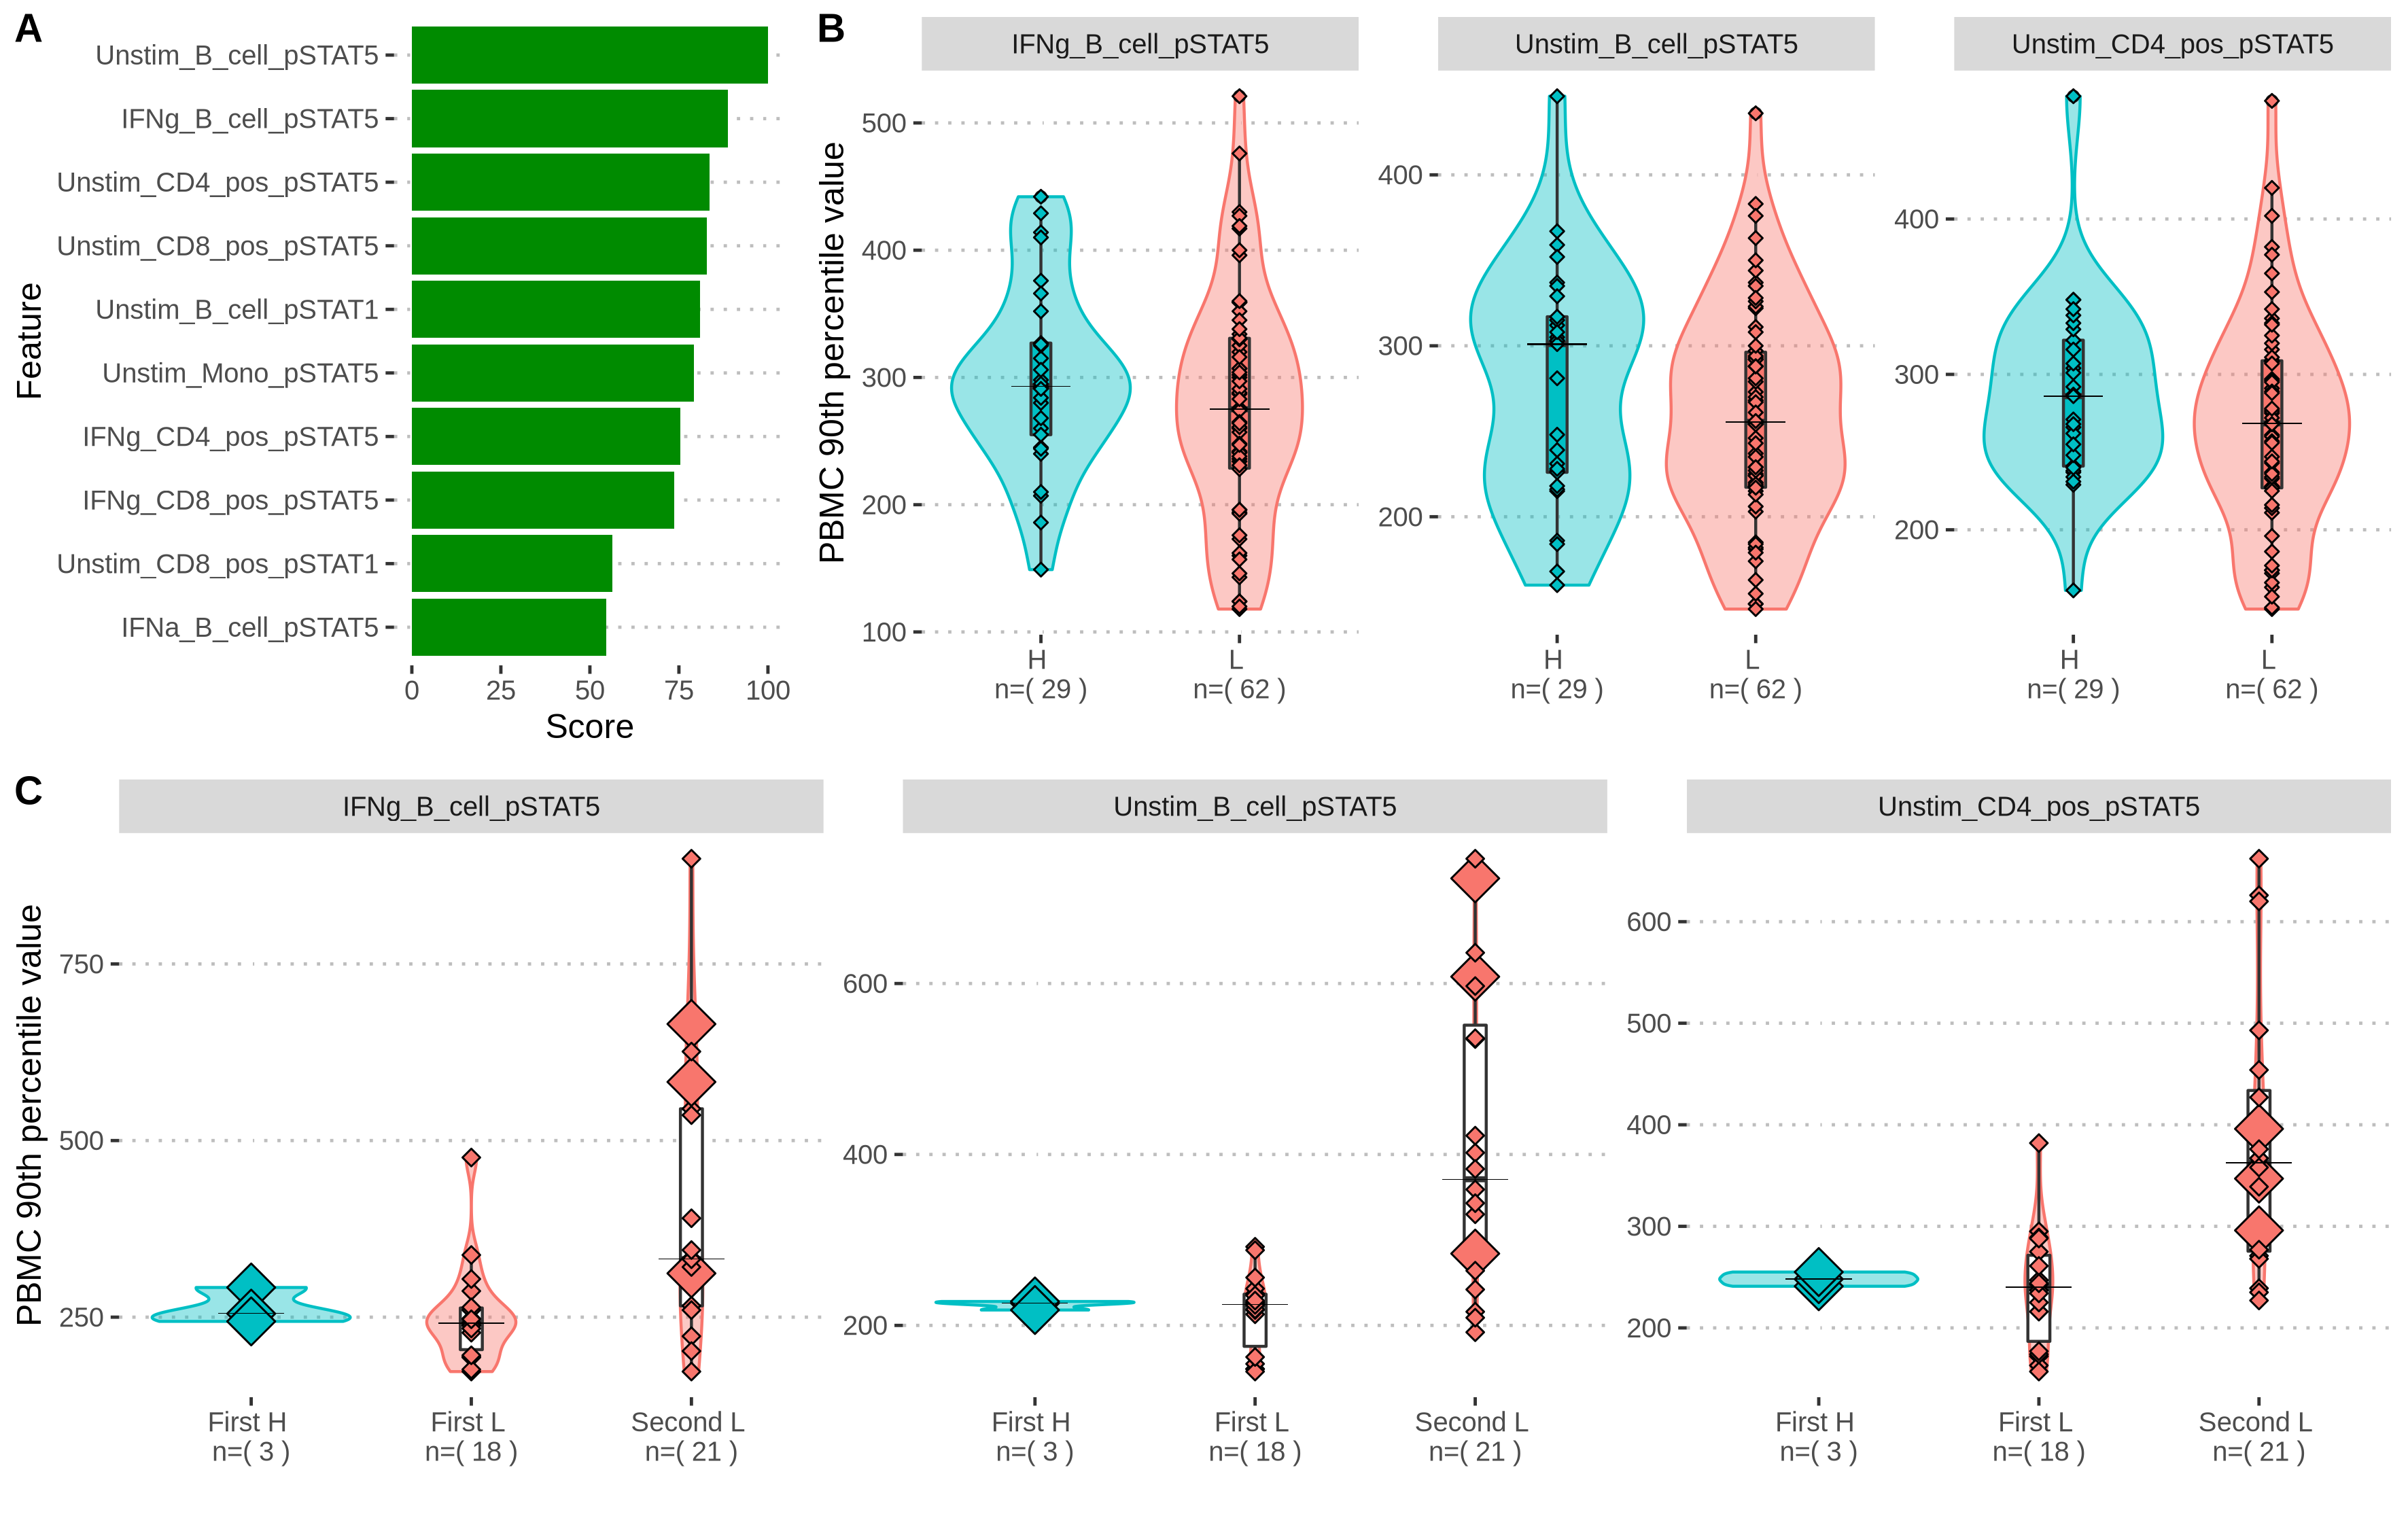
\includegraphics[width=\textwidth]{dataset1_nb_feature_exploration}
    \caption{dataset1-nb-feature-exploration}
    \label{fig:dataset1-nb-feature-exploration}
\end{figure}

Firstly, the top ranked feature in dataset 14 was the phosphorylated STAT5 transcription factor in unstimulated B cells \autorefsub{fig:dataset1-nb-feature-exploration}{A}. However, the difference in the value of this feature between the high and low vaccine responders was not found to be significant at FDR $<$ 0.01 \autorefsub{fig:dataset2-nb-feature-exploration}{B}. In contrast, the other two features, IFNg stimulated B-cell phosphorylated STAT5 and CD4 T cell phosphorylated STAT5, were found to be significantly greater in the high responder group (FDR $<$ 0.01). A correlation analysis of all features showed that different STAT protein formed positively correlated clusters as expected \autoref{fig:cor-dataset1} (p < 0.0001). Further, the most important feature had slight negative correlations (pearson's r from -0.2 to -0.5) to a set of stimulated STAT1 cell responses (p < 0.0001 after BH adjustment). The second most important feature has similar correlations as the first, likely since they are both B-cell STAT5 features. Lastly, the unstimulated CD4 positive phenotype T-cells STAT5 phosphorylation also belonged in the same cluster as the previous B-cell features. These correlations might indicate an interaction between the STAT5 and STAT1 phosphorylation in response to a vaccine.

\begin{figure}[htpb]
    \centering
    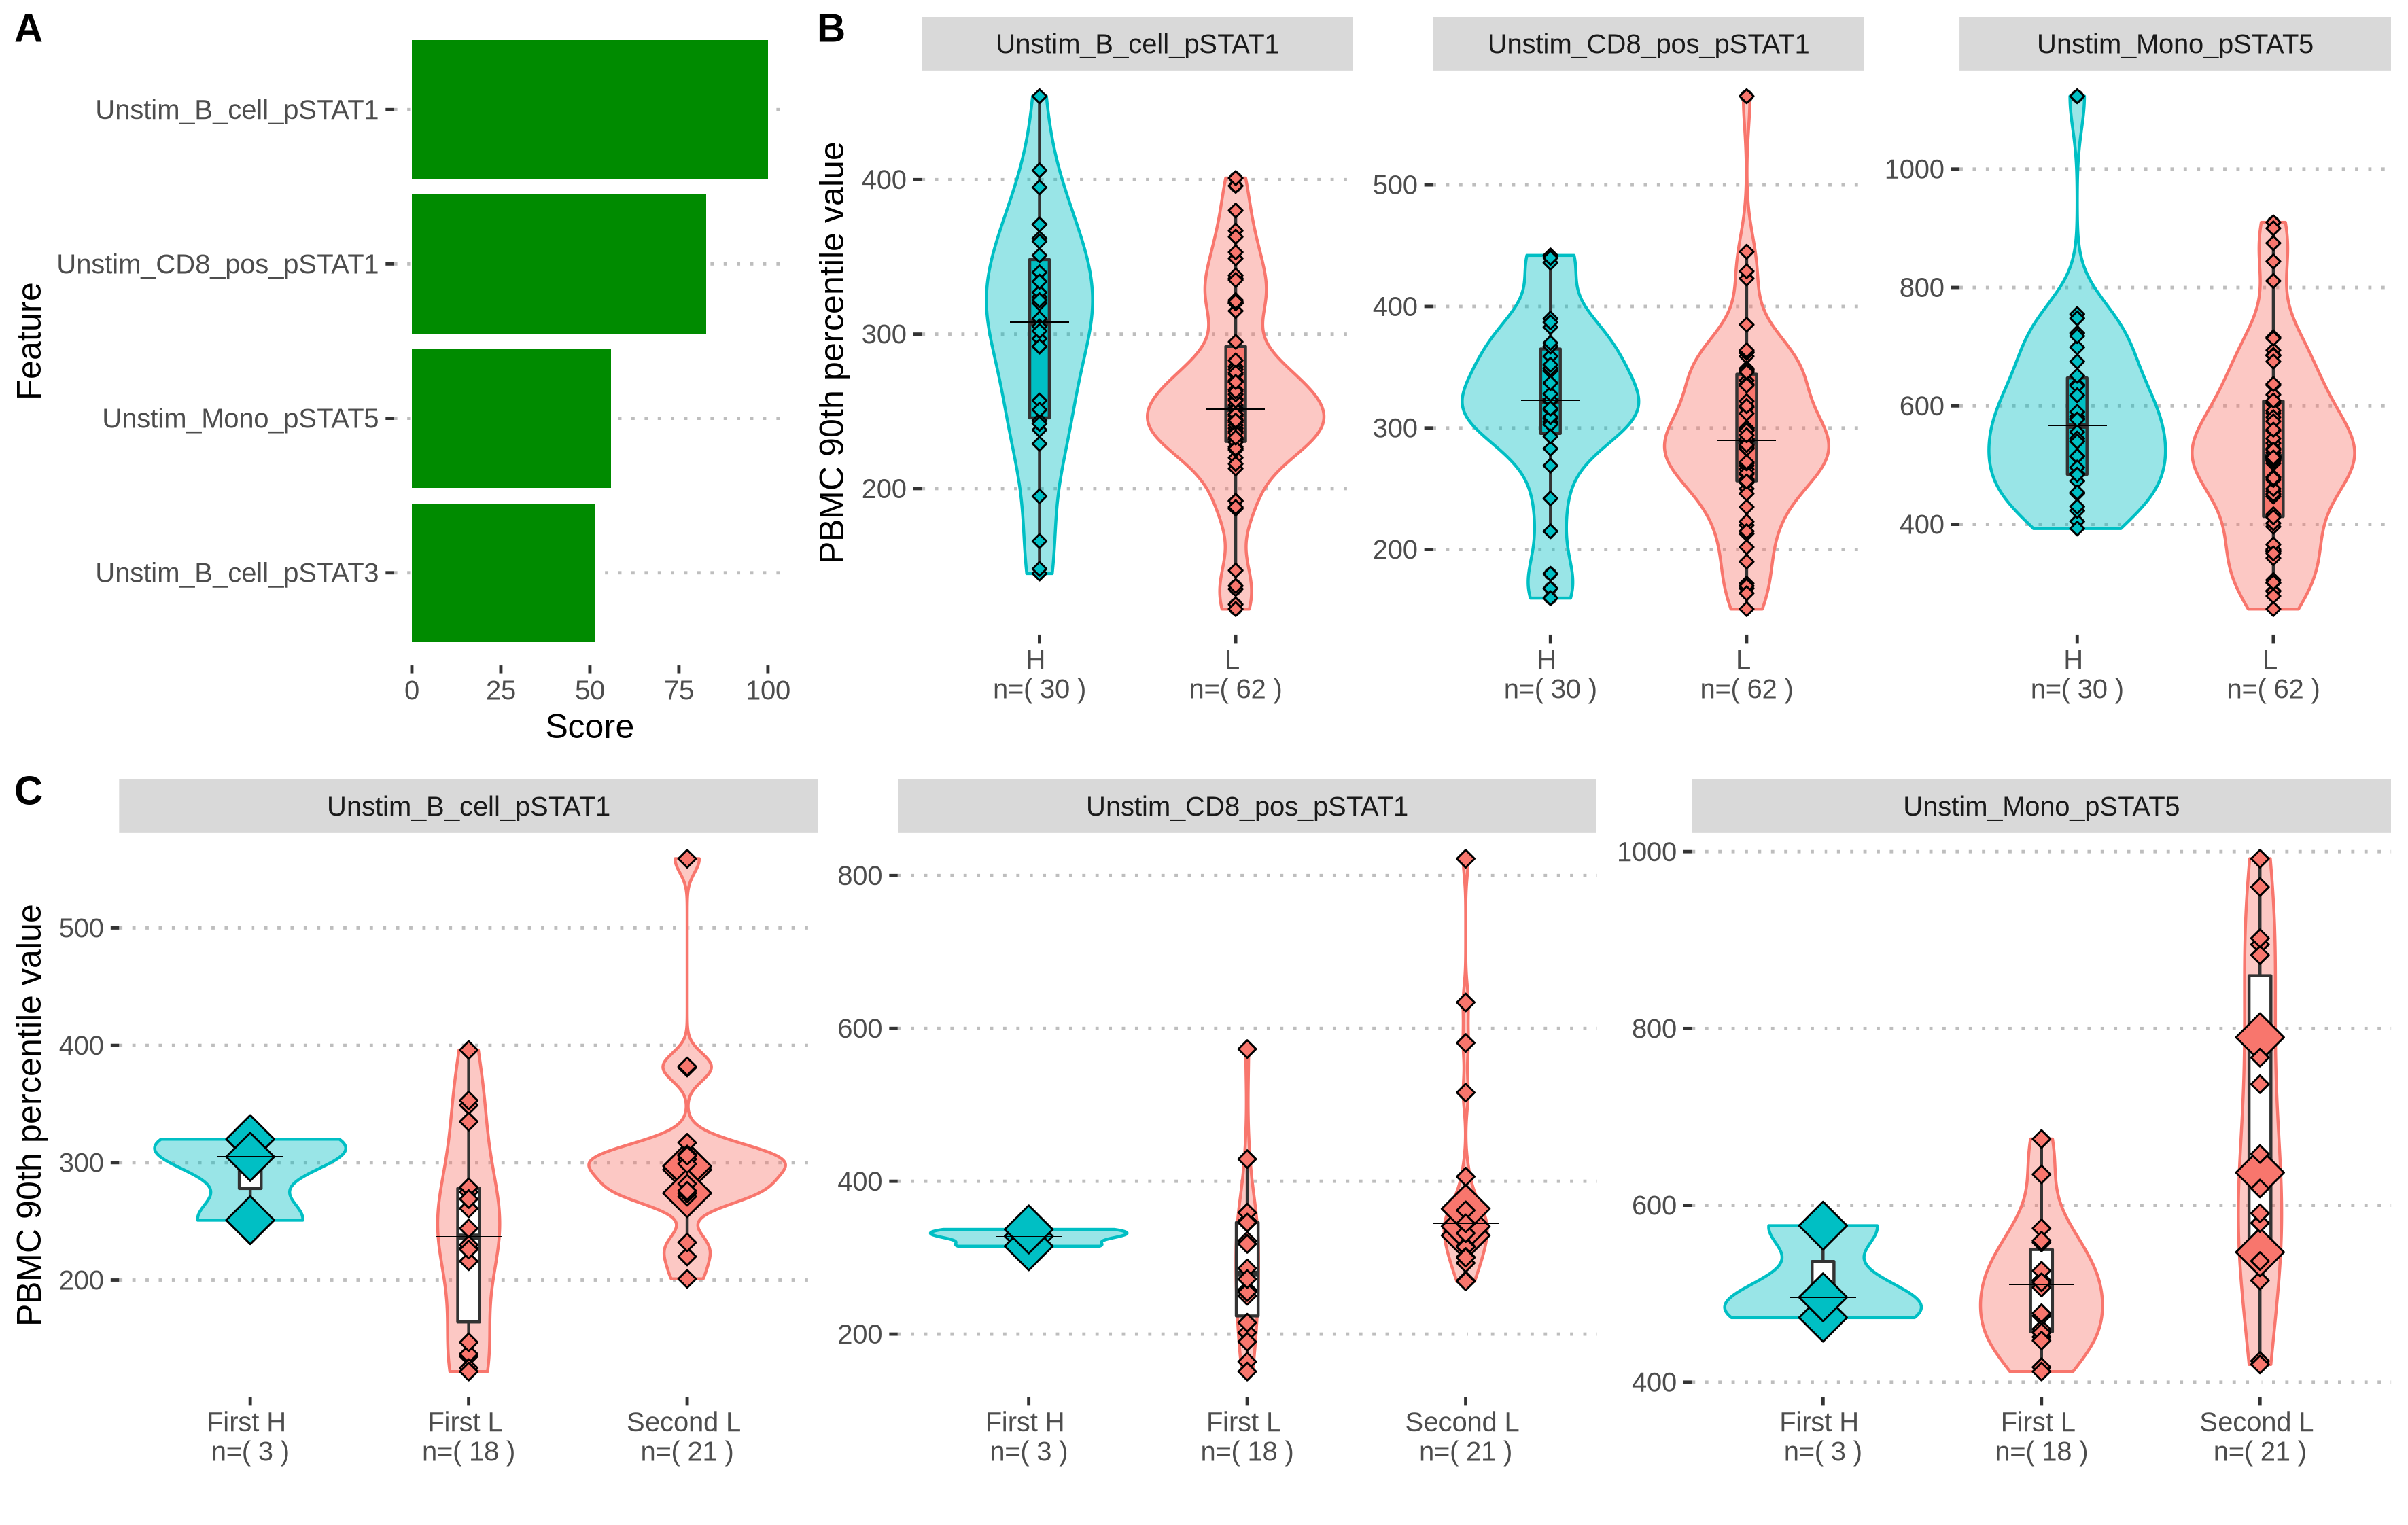
\includegraphics[width=\textwidth]{dataset2_nb_feature_exploration}
    \caption{dataset2-nb-feature-exploration}
    \label{fig:dataset2-nb-feature-exploration}
\end{figure}

Secondly, in dataset 16 there were only four features that had a variable importance score greater than 50 \autorefsub{fig:dataset2-nb-feature-exploration}{A}. The top two features were phospohorylated STAT1 in unstimulated B-cells and phosphorylated STAT1 in unstimulated CD8 T-cells. However, only the B-cell feature was found to be significantly greater in the positive class (FDR \(< 0.01\)) \autorefsub{fig:dataset2-nb-feature-exploration}{B}. The B-cell STAT1 feature correlated positively with both unstimulated CD8 and CD4 STAT1 phosphorylation (pearson's r= 0.7 and 0.4, p \(< 0.001\)), and there were mild negative correlations with interferon gamma stimulated monocyte STAT3 and STAT5 phosphorylation (pearson's r= 0.3 and 0.2, p \(< 0.001\)) \autoref{fig:cor-dataset2}.

\subsection{Repeat vaccination effect on identified features}

Firstly, in the \secondvis of both datasets there were outliers (donors had a value greater than 1000) and negative values. In this work these were left out, since outliers made the pattern unclear and the negative values were considered as nonsensical values.

\begin{figure}[htpb]
    \centering
    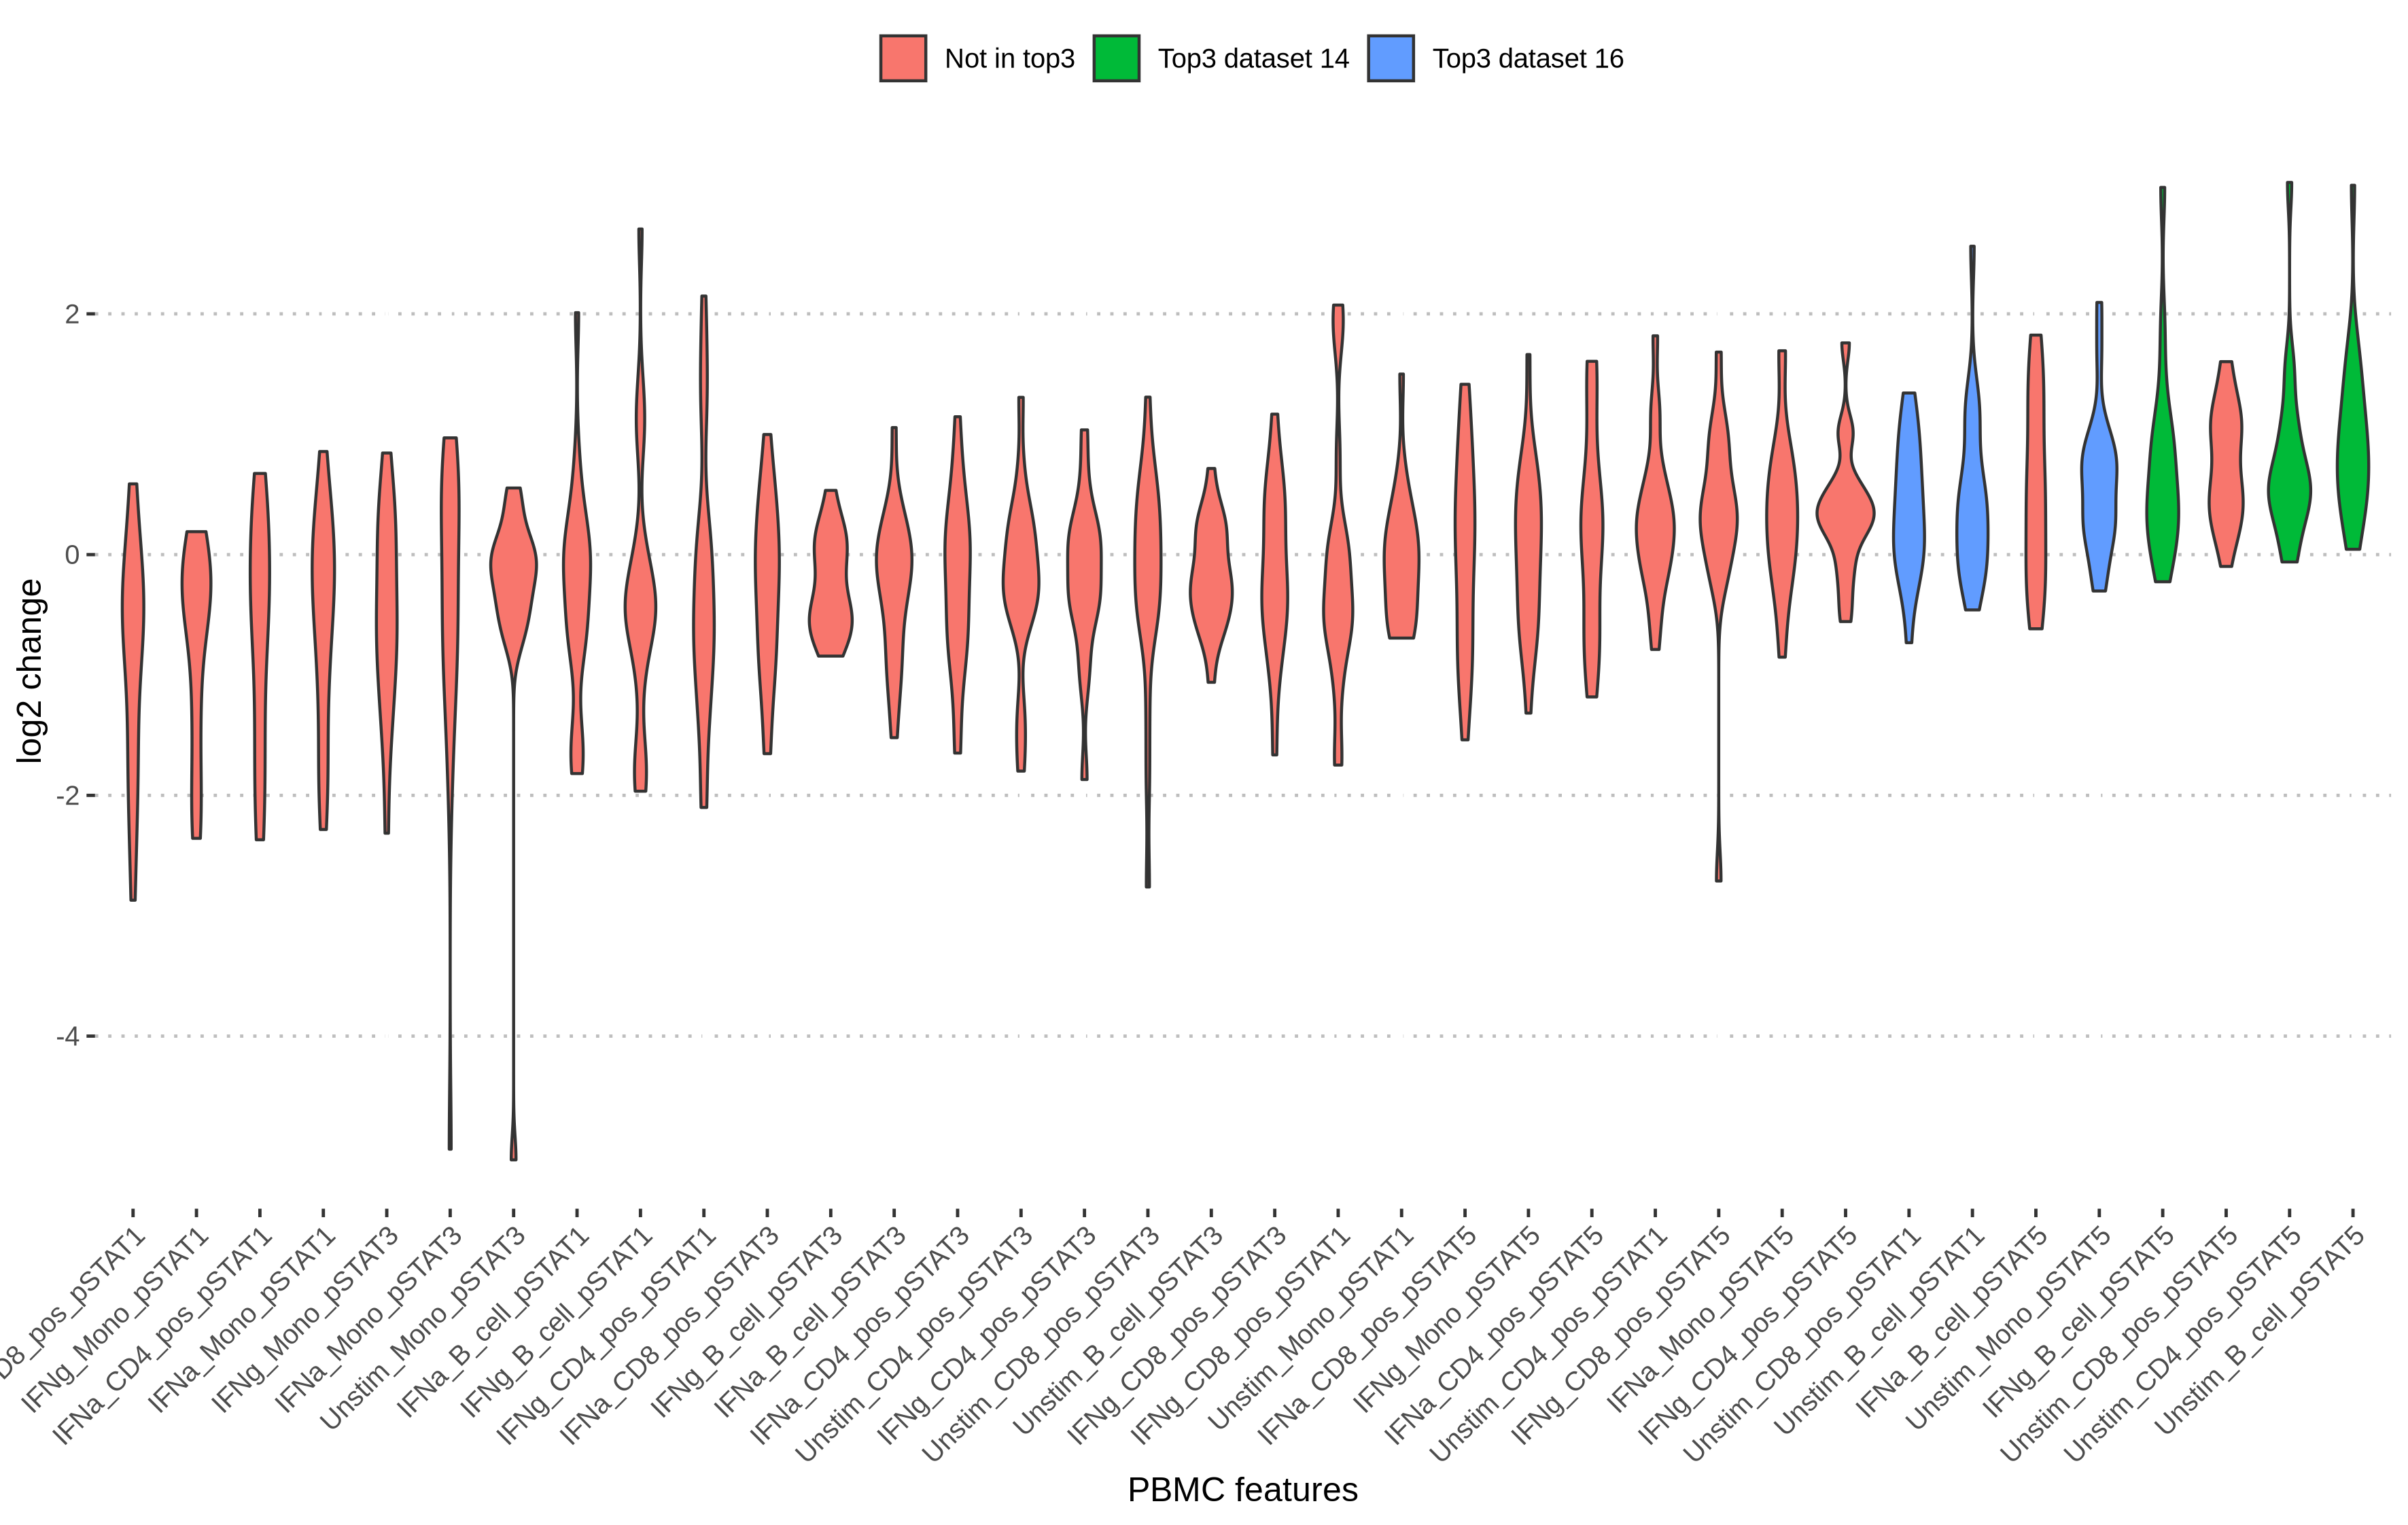
\includegraphics[width=\textwidth]{second_visit_change1}
    \caption{second-visit-change1}
    \label{fig:second-visit-change1}
\end{figure}

To see how a repeat vaccination affects immune cell signaling, the distribution of the top three features of dataset 14 were compared to their distribution when measured in a subsequent influenza season \autorefsub{fig:dataset1-nb-feature-exploration}{C}.
In the 21 donors that had a second measurement of the features in another influenza season that were not left out (outliers and nonsensical values) there was the consistent pattern that the high responders were classified as low responders in their second visit \autorefsub{fig:dataset1-nb-feature-exploration}{C}.
Although, overall the feature values were consistently greater in the \secondvis \autorefsub{fig:dataset1-nb-feature-exploration}{C, enlarged diamonds}.
Thus, vaccination might increase activity in general signaling pathways of PBMC in subsequent influenza seasons, but the classification does not reflect this as increasing influenza antibody response.
One possibility is that the donor was classified as low responder due to a lack of response to one strain of virus in the vaccine administered in the repeat visit, not necessarily to all strains \autoref{fig:classInconsistent}.

To explore the overall change in the features of dataset 14 between the first and subsequent in influenza seasons the distribution of changes for donors were visualised and ordered by mean of log2 change (negative values were removed) \autoref{fig:second-visit-change1}.
The overall trend that appeared was that the unstimulated PBMCs had higher values upon a repeated visit.
And, in general STAT5 features increased in value. The values that contributed the most to the model discriminating between high and low responders in the \firstvis also increased the most in a repeat visit.
Although, there are outliers that increased a lot in the subsequent influenza season \autoref{fig:second-visit-change1}.

On dataset 16 two of the top three features had similar distributions to the \firstvis \autorefsub{fig:dataset2-nb-feature-exploration}{C}.
In contrast, unstimulated monocyte cells had higher STAT5 phoshporylation in the subsequent influenza season \autorefsub{fig:dataset2-nb-feature-exploration}{C}.
Further, the same three donors that were classified as high responders in the \firstvis and as low responders in the \secondvis as in dataset 14 \autorefsub{fig:dataset1-nb-feature-exploration}{C} had increased monocyte cell STAT5 phosphorylation \autorefsub{fig:dataset2-nb-feature-exploration}{C, enlarged diamonds}.
Lastly, the top three features of the model trained on dataset 14 also belonged to those that increased the most between the \firstvis and \secondvis \autoref{fig:second-visit-change1}.

\section{Discussion and conclusion}

In this work we gave a brief introduction into influenza vaccination and how vaccine responses are measured, described the \flup database, and applied a similar data mining method as in \spaper and additionally explored the available repeat vaccination data.
The \flup database made it possible to study vaccine responses by providing a classification of donors into high or low responders based on measured antibody level before and after vaccination.
Further, it combined and preprocessed data from multiple clinical studies in an accessible database format.
This resulted in a wide variety of data on immune cell populations, serum signaling molecules, and cell signaling activity that is suitable for studying immune correlates to vaccine responses using data mining method.
We applied a procedure as described by the authors of \flup in \spaper, wrapper feature selection using multiple models trained on interesting data subsets of \flup. Using this procedure we then explored selected features and how they changed in subsequent influenza seasons.
It was found that STAT5 related signaling features correlated with a vaccine response and increased the greatest amount in subsequent influenza seasons.

Initially, the idea was to focus on building accurate predictors of vaccine response by training models including constructed features based on repeat vaccination. However, during the data understanding phase of this project it became clear that \flup contains only complete classifications in the \firstvis.
Instead, the objective was revised to explore the available data on repeat vaccination using models trained on \firstvis data from a selection of clinical studies that received the same vaccine, as done in \spaper.
Overall, during the data understanding phase it became clear that \flup is not suitable for predicting vaccine response with high accuracy, since data is combined from multiple studies and years.
This means using donors/rows from different years and studies creates highly sparse predictors.
Consequently, using \flup data requires selecting small datasets without missing values, this only slightly increases the available example measurements of features by combining data from different studies.
Further, the available data on repeat vaccinations is limited to mostly one clinical study, and in repeat visits there is often no classification making it impossible to train models using repeat vaccination data.

During the data understanding phase we also found that classification is missing in a lot of cases.
Further, we identified an inconsistency in the classification data presented in \flup.
However, this is likely due to the fact that the before and after antibody titer against individual influenza strains in the vaccine is not completely available in the database and not because the classification is incorrect.
Thus to check the classification quality it is necessary to study the raw data and scripts used to generate the database, which is considered out of the scope of this work.

The data preparation and modeling phases included selecting the data that was most suitable for training models and studying repeat vaccinations.
We started with the initial data used in \spaper and also collected repeat vaccination data for the donors in this dataset.
To deal with the sparse data the mulset algorithm was applied to generate twenty small but complete datasets, the three datasets that had the highest amount of donors that received a repeat vaccination were then chosen for modeling and further analysis.
Four models were built all three datasets, but models with fair discriminative ability were built only on dataset 14 and 16.

The features in dataset 14 and 16 were all from the phospho-flow cytometry phosphorylation assay, from them we used the models to identify features correlated with a high vaccine response.
We found that STAT5 phosphorylation in immune cells from different lineages was associated with a high vaccine response and was increased in subsequent influenza seasons.
However, further study of this result is considered out of the scope of this work where the focus lies on the application of data science tools.
Instead, we show here that data mining methods described in \spaper can be replicated to answer research questions using complex clinical datasets.

The objectives defined before selecting the data and starting the data preparation and modeling phase of the project were:
\begin{itemize}
        \item What kind of studies can be done using the \flup database?
        \item What immunological factors correlate to a vaccine responses?
        \item What is the effect of repeat vaccination?
\end{itemize}

In summary, we provided insight into which studies can be done using the \flup database by describing the experimental data tables of \flup.
It became clear that \flup is suitable for correlating immunological features with a vaccine response by selecting small complete datasets, but that the possibility of combining large data across years and different studies is limited in \flup.
Additionally, we found that classifications are not available in a great amount of data points limiting the sample size for classification studies.
Further, we identified a group of immune cells from different lineages that had increased phosphorylation activity correlated to vaccine response and found that this increase was present in subsequent influenza seasons.

\section{Materials and methods}

\subsection{Data collection}

By following the guide on the \href{https://github.com/LogIN-/fluprint}{FluPrint Github Repository} the MySQL
server was set up.
All file paths mentioned refer to the github repository of this project which can be found below.

In this work the FluPrint github was first added as a submodule.
This module provides the php scripts to import raw data csv's into the MySQL database.
The operating system and versions of php and MySQL used in this work were OSX "Big Sur" (on Mac Book air 2017), php 7.3.24 (built-in mac version), and MySQL 8.0.23 (homebrew).

In the \href{https://github.com/LogIN-/fluprint}{guide} the dependencies to run
the php import script were installed first. This was also done in this work,
except that the hash-file verification step was skipped.

After the php dependencies were installed the MySQL server was started. By
default homebrew recommends to use the \lstinline{homebrew services [option] [SERVICE]} command to start the MySQL server. However, in this work the server
is started using \lstinline{mysql.server start} which provides a socket that
was symlinked using \lstinline{sudo ln -s /tmp/mysql.sock /var/mysql/mysql.sock}. This was done to prevent an error
(\href{https://stackoverflow.com/questions/15016376/cant-connect-to-local-mysql-server-through-socket-homebrew/18090173}{StackOverflow: cant connect to local mysql server through socket homebrew}) thrown
by the php import scripts. Before the import scripts were run a user was added to the
MySQL server and a database was created \ref{lst:addUser}, the password type had to be \lstinline{mysql_native_password}
(\href{https://stackoverflow.com/questions/62873680/how-to-resolve-sqlstatehy000-2054-the-server-requested-authentication-metho}{how to resolve [SQLSTATEHY000] 2054 the server requested authentication method.}).

\begin{lstlisting}[language=sql, caption=Adding user and database to sql server, label={lst:addUser}]
mysql> CREATE USER 'mike'@'localhost' IDENTIFIED BY ';lkj';
mysql> GRANT ALL PRIVILEGES ON * . * TO 'mike'@'localhost';
mysql> ALTER USER 'mike'@'localhost' IDENTIFIED WITH mysql_native_password BY 'mike';
mysql> CREATE DATABASE fluprint;
\end{lstlisting}

The databasename, the username, and password were added to the
\lstinline{config/configuration.json} of the FlruPrint github module. At this
point the configuration for the php import scripts was finished, and the raw
data downloaded in \lstinline{data/upload} were imported in the MySQL server
using \lstinline{php bin/import.php}.

\subsection{Statistical methods}

\subsubsection{Data selection}

In this work immunological features correlating to a vaccine response were identified using wrapper based feature selection on data from the \flup SQL database.
Suitable datasets without missing values were generated using the \href{https://cran.r-project.org/web/packages/mulset/index.html}{R package mulset}, as described in the data preparation section.
These datasets were split into training and test splits using the createDataPartition function from the R package \href{https://topepo.github.io/caret/}{caret}.
As described in the data preparation and selection sections, datasets were not considered if the test set had less than 10 donors.
Lastly, from the generated datasets the number of donors in the \secondvis was used to choose datasets for further analysis. The \secondvis data was obtained from the database by a query that is avalaible in the github repository of this project.

\subsubsection{Model training, evaluation, exploration}

Standard procedure were used for model training, models were trained only on the training datasets using 10-fold cross-validation that was repeated two times.
The test data was used only as an independent dataset to estimate how much the model overfits on the training data.
Model training itself was done using the \href{https://topepo.github.io/caret/}{caret} R package function train.
Additionally, parameters were chosen based on the highest cross-validated accuracy automatically train function.

Variable importance of the models generated by the \href{https://topepo.github.io/caret/}{caret} package was generated by the function varImp from the same package.
This uses model specific feature contribution statistics and ranks them from most important to not important on a scale from 0 to 100, for example for the naive bayes model it uses the class conditional probabilities of features.

Confusion matrix metrics were generated using the \href{https://cran.r-project.org/web/packages/MLeval/index.html}{MLeval} R package which accepts caret objects and computes metrics in a table format as shown in the model evaluation section.
Additionally, the test AUC was calculated with another R packages called \href{https://cran.r-project.org/web/packages/pROC/pROC.pdf}{pROC}.

Correlation plots of the features from the selected datasets 14 and 16 were made using the R package \href{https://cran.r-project.org/web/packages/corrplot/vignettes/corrplot-intro.html}{corrplot}.

\subsubsection{Significance tests}

To see if features identified by the best classifier trained on datasets 14 and 16 had different distribution in between the two classes the significance analysis of micro arrays (SAM) at a FDR \(<\) 0.01 was used in R.
P values for all correlations shown in the correlation plots below were calculated using an R package, and only correlations with a p-value less than 0.001 were shown.

\subsection{Code and data availability}

The code and data belonging to this project can be found in the \href{https://github.com/Vinkage/fluprint_exploration}{github repository}.
The repository contains the directories \lstinline{bussiness_understand}, \lstinline{data_understanding} and \lstinline{data_preparation_modeling} which contain all the \LaTeX source files for what was written during the project.
However, the source files for the final pdf deliverable that is to be graded are in the \lstinline{deliverable} directory.
The directory \lstinline{csv} contains all the flat data files that were generated in this work, \lstinline{queries} contains the SQL source files.
As mentioned above, the import script for constructing the database is added as a submodule called \lstinline{fluprint}.
Other files and directories are data files used in the latex source files.

\printbibliography

\begin{appendices}

    \section{Correlation plots}

\begin{figure}[htpb]
    \centering
    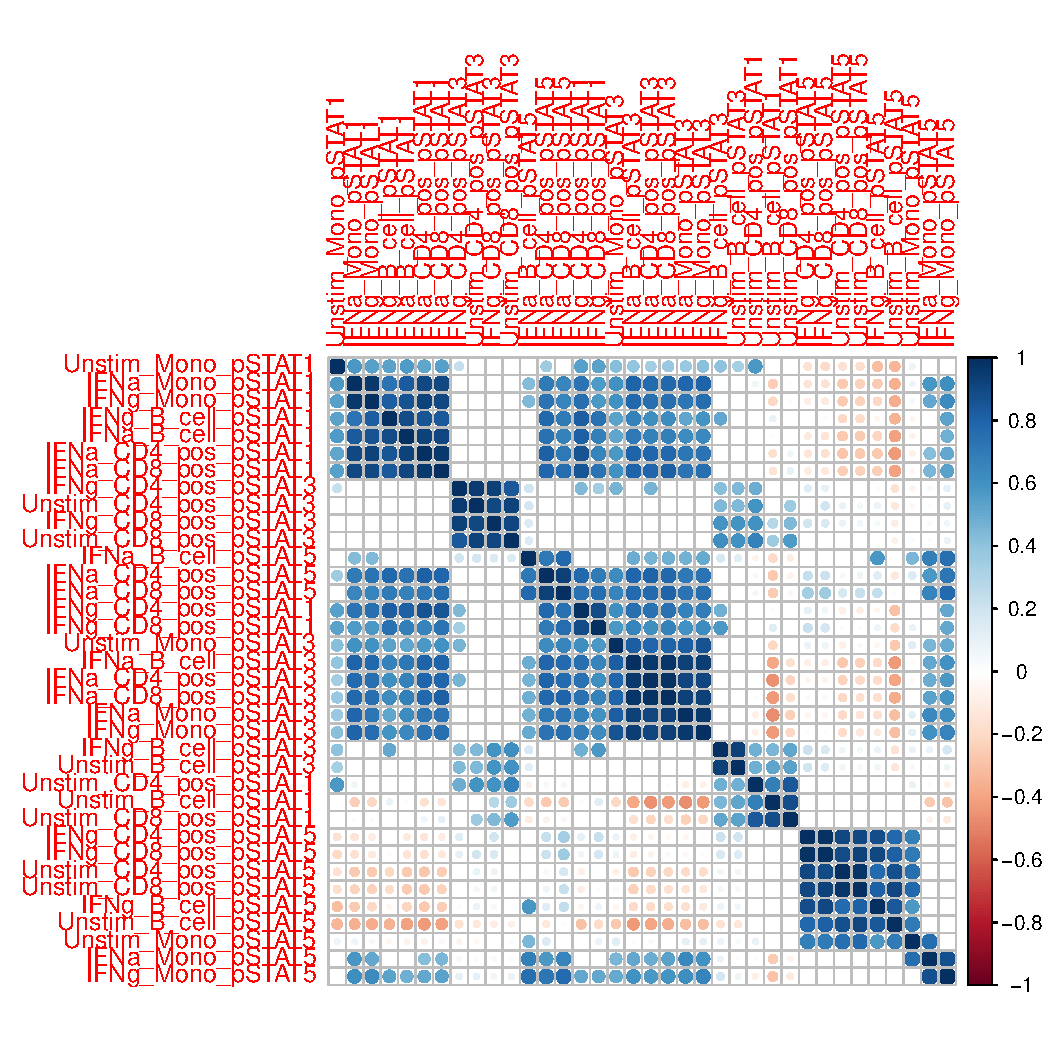
\includegraphics[width=\textwidth]{cor_dataset1}
    \caption{cor-dataset1}
    \label{fig:cor-dataset1}
\end{figure}

\begin{figure}[htpb]
    \centering
    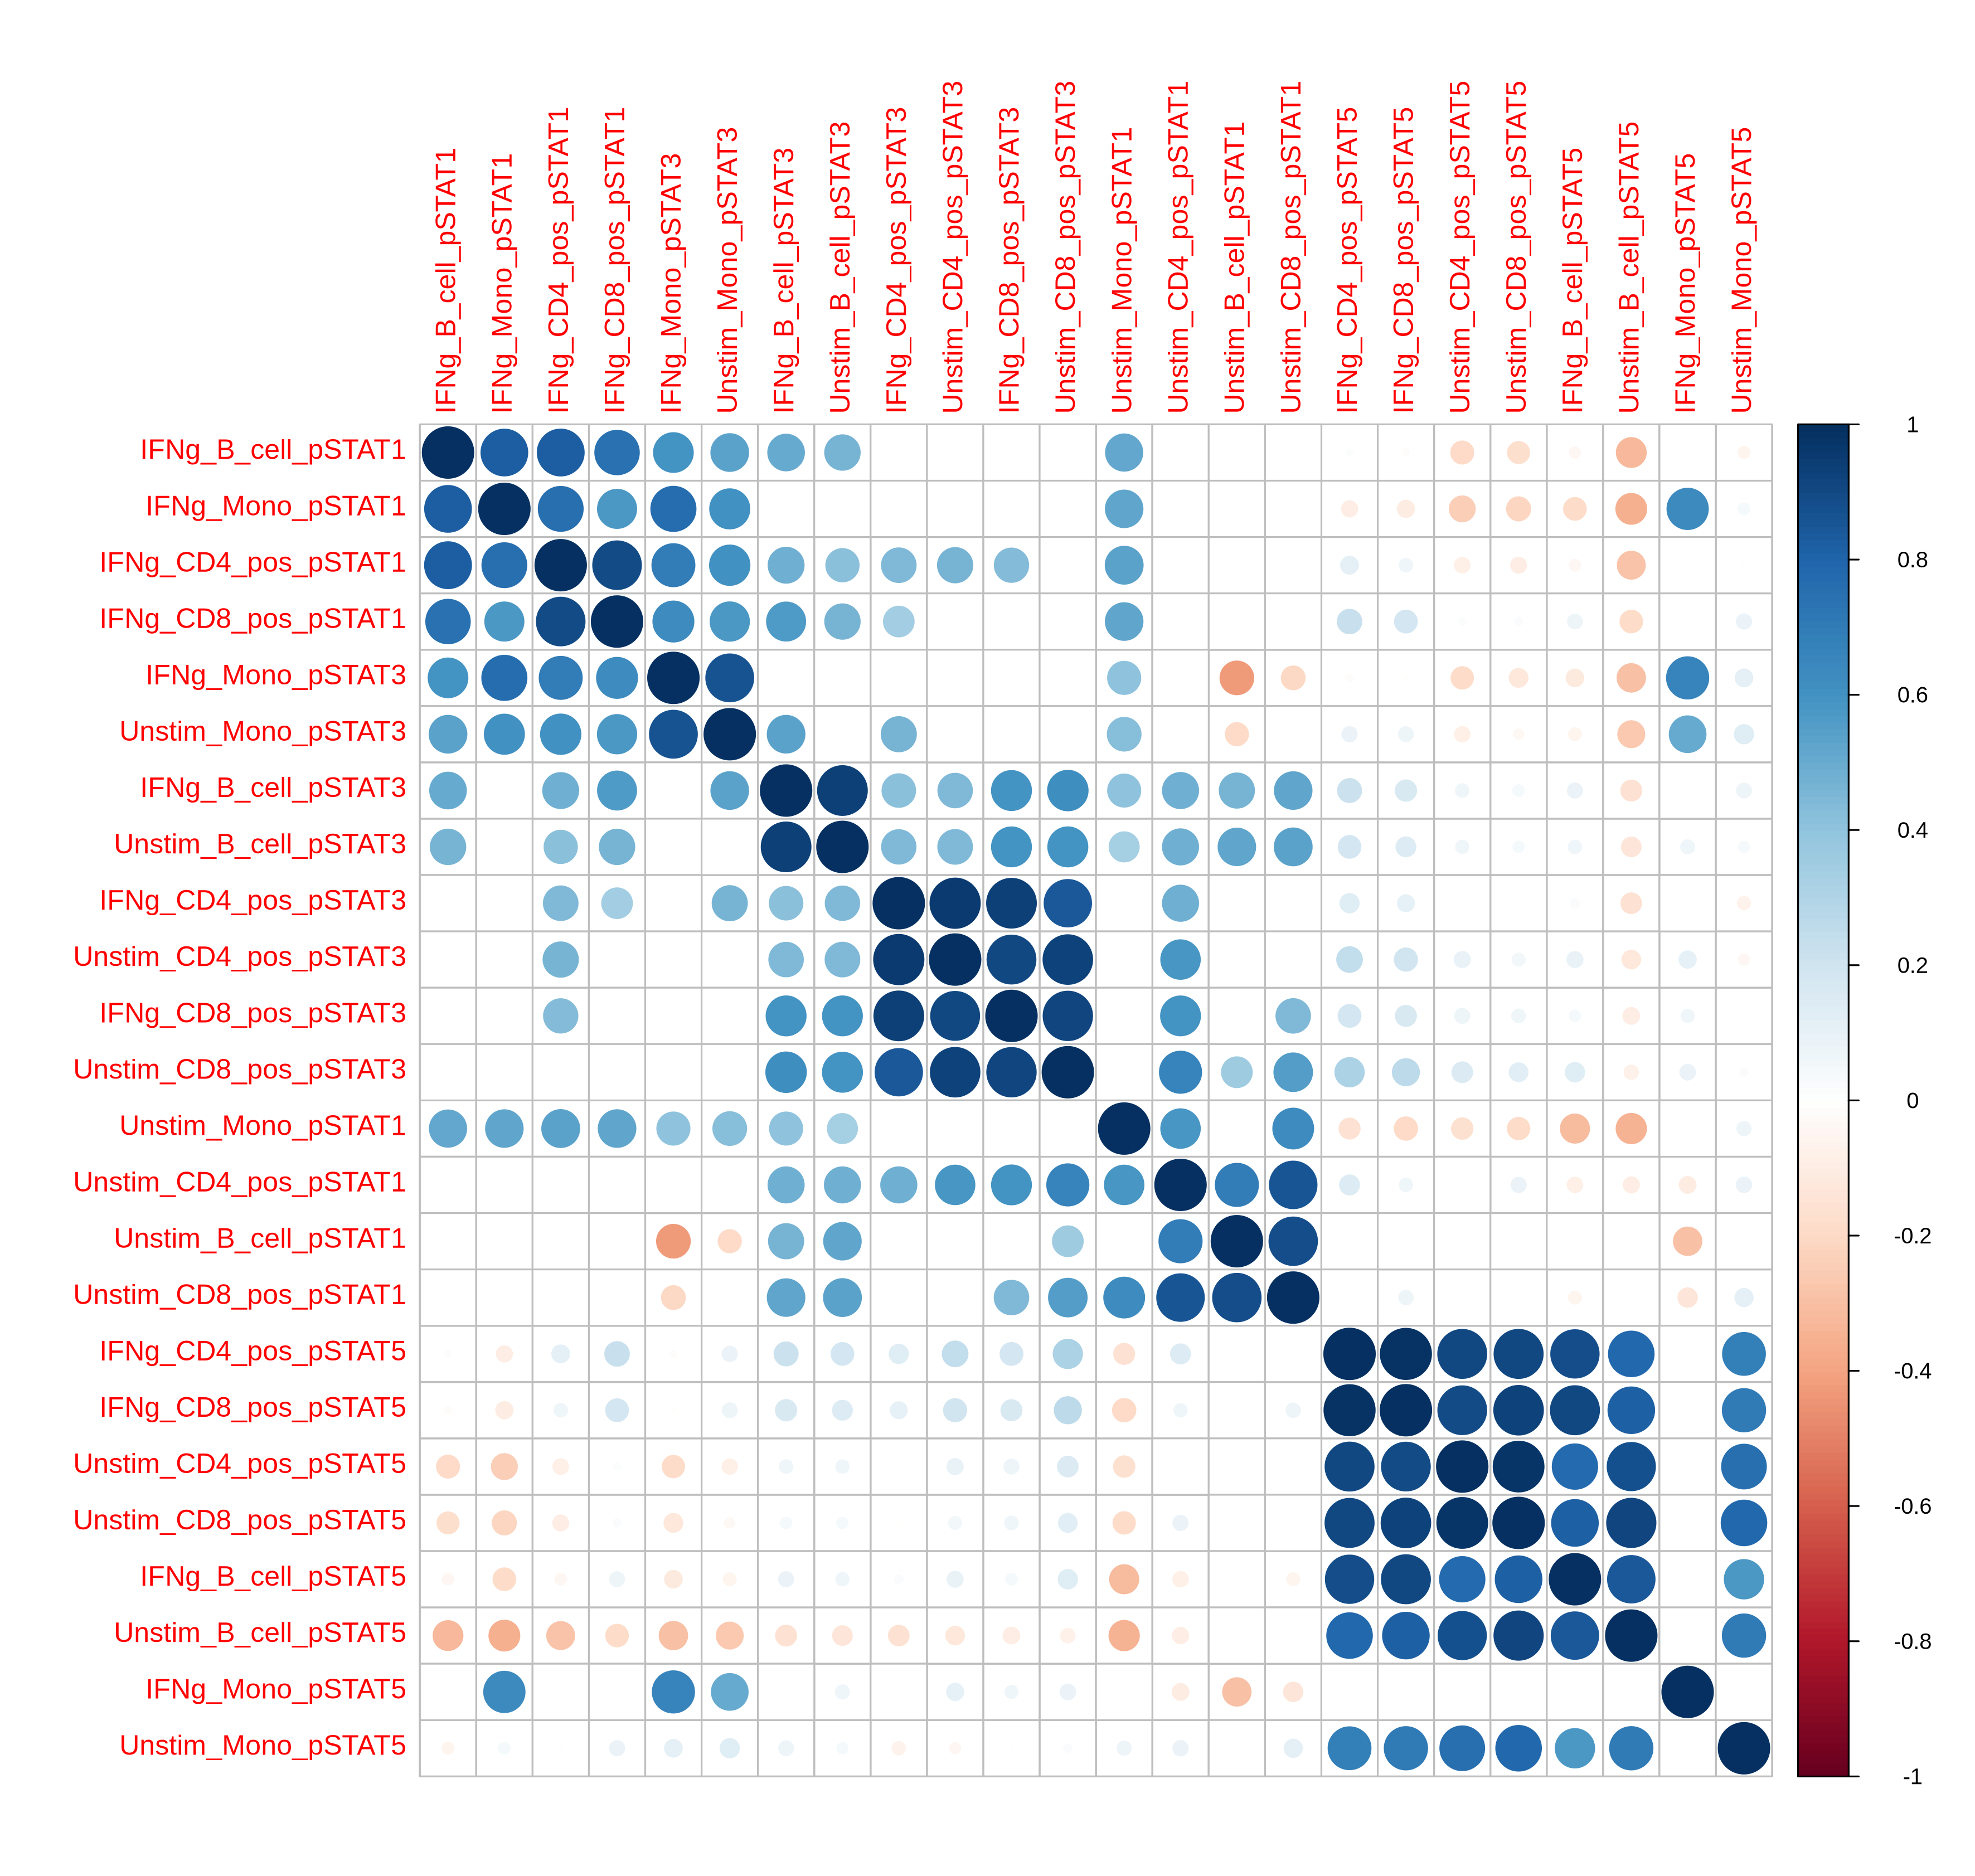
\includegraphics[width=\textwidth]{cor_dataset2}
    \caption{cor-dataset2}
    \label{fig:cor-dataset2}
\end{figure}

    \section{mulset algorithm}

\begin{figure}[htpb]
    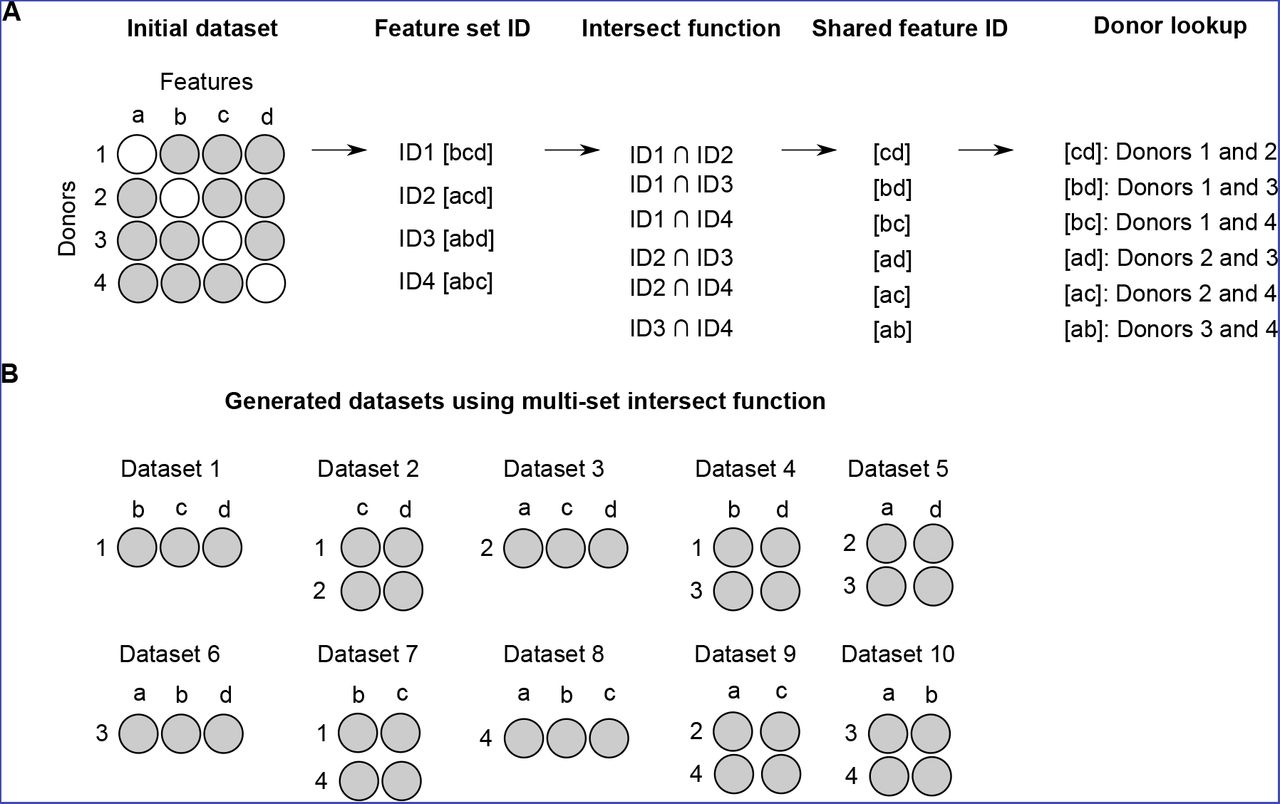
\includegraphics[width=\textwidth]{F2.large}
    \caption{\textbf{taken from original work}}\label{fig:mulsetAlg}
\end{figure}

\begin{table}[htpb]
\addtolength{\leftskip} {-2cm} % increase (absolute) value if needed
\addtolength{\rightskip} {-2cm} % increase (absolute) value if needed
\begin{tabular}{rrrrrlrllrrl}
\toprule{}
donor\_id & study & age & outcome & year & type & hai\_response & name & data\_name & assay & data & dup\\
\midrule{}
285 & 18 & 9.47 & 0 & 2009 & pre & 1 & CD4+ T cells & CD4\_pos\_T\_cells & 13 & 33.8 & TRUE\\
285 & 18 & 9.47 & 0 & 2009 & pre & 1 & CD4+ T cells & CD4\_pos\_T\_cells & 13 & 34.1 & TRUE\\
285 & 18 & 9.47 & 0 & 2009 & pre & 1 & CD4+ T cells & CD4\_pos\_T\_cells & 13 & 34.3 & TRUE\\
285 & 18 & 9.47 & 0 & 2009 & pre & 1 & CD4+ T cells & CD4\_pos\_T\_cells & 13 & 33.0 & TRUE\\
\bottomrule{}
\end{tabular}
    \caption{}\label{tbl:exampleDuplicate}
\end{table}



    \section{Query that generates initial \simon data}
\begin{lstlisting}[language=sql, caption=Query of initial SIMON data, label={lst:QueryTemplate}]
SELECT donors.id                        AS donor_id,
       donor_visits.age                 AS age,
       donor_visits.vaccine_resp        AS outcome,
       experimental_data.name_formatted AS data_name,
       experimental_data.data           AS data
FROM   donors
       LEFT JOIN donor_visits
              ON donors.id = donor_visits.donor_id
                 AND donor_visits.visit_id = 1
       INNER JOIN experimental_data
               ON donor_visits.id = experimental_data.donor_visits_id
                  AND experimental_data.donor_id = donor_visits.donor_id
WHERE  donors.gender IS NOT NULL
       AND donor_visits.vaccine_resp IS NOT NULL
       AND donor_visits.vaccine = 4
ORDER  BY donors.study_donor_id DESC
\end{lstlisting}

    \section{Full description of FluPrint clinical studies}
\fptable{studies_table}{.7}
{Reference table of clinical studies}
{Clinical study ID used (but remapped) in the database, age information,
vaccine type information, and assay data types of clinical studies are in the
rest of the columns.}
{tbl:studiesDesc}


    \section{Remaps used in the \flup}

    \begin{table}[htpb]
        \begin{tabular}{lll}
            \toprule{}
            Vaccine received & Vaccine type ID & Vaccine type name \\
            \midrule{}
            FluMist IIV4 0.2 mL intranasal spray & 1 & Flumist \\
            FluMist Intranasal spray & 1 & Flumist \\
            FluMist Intranasal Spray 2009–2010 & 1 & Flumist \\
            FluMist Intranasal Spray & 1 & Flumist \\
            Flumist & 1 & Flumist \\
            Fluzone Intradermal-IIV3 & 2 & Fluzone Intradermal \\
            Fluzone Intradermal & 2 & Fluzone Intradermal \\
            GSK Fluarix IIV3 single-dose syringe & 3 & Fluarix \\
            Fluzone 0.5 mL IIV4 SD syringe & 4 & Fluzone \\
            Fluzone 0.25 mL IIV4 SD syringe & 5 & Paediatric Fluzone \\
            Fluzone IIV3 multi-dose vial & 4 & Fluzone \\
            Fluzone single-dose syringe & 4 & Fluzone \\
            Fluzone multi-dose vial & 4 & Fluzone \\
            Fluzone single-dose syringe 2009–2010 & 4 & Fluzone \\
            Fluzone high-dose syringe & 6 & High Dose Fluzone \\
            Fluzone 0.5 mL single-dose syringe & 4 & Fluzone \\
            Fluzone 0.25 mL single-dose syringe & 5 & Paediatric Fluzone \\
            Fluzone IIV3 High-Dose SDS & 6 & High Dose Fluzone \\
            Fluzone IIV4 single-dose syringe & 4 & Fluzone \\
            Fluzone High-Dose syringe & 6 & High Dose Fluzone \\
            \bottomrule{}
        \end{tabular}
        \caption{Remaps of vaccine type relevant to to the clinical studies
        reference table \autoref{tbl:studiesDesc}, and the section on the donor
        visits table.}\label{tbl:remapVaccine}
    \end{table}

    \begin{table}[htpb]
        \begin{tabular}{ll}
            \toprule{}
            Original & Remapped \\
            \midrule{}
            No& 0 \\
            Yes& 1 \\
            IIV injection/im& 2 \\
            Doesn’t know/doesn’t remember/na/does not remember& 3 \\
            LAIV4 intranasal/laiv\_std\_intranasal/laiv\_std\_ intranasal/nasal/intranasal& 4 \\
            \bottomrule{}
        \end{tabular}
        \caption{caption}\label{tbl:remapHistory}
    \end{table}

    \begin{table}[htpb]
        \begin{tabular}{ll}
            \toprule{}
            Original & Remapped \\
            \midrule{}
            CMV EBV & 1 \\
            Other immunoassay & 2 \\
            Human Luminex 62–63 plex & 3 \\
            CyTOF phenotyping & 4 \\
            HAI & 5 \\
            Human Luminex 51 plex & 6 \\
            Phospho-flow cytokine stim (PBMC) & 7 \\
            pCyTOF (whole blood) pheno & 9 \\
            pCyTOF (whole blood) phospho & 10 \\
            CBCD & 11 \\
            Human MSD 4 plex & 12 \\
            Lyoplate 1 & 13 \\
            Human MSD 9 plex & 14 \\
            Human Luminex 50 plex & 15 \\
            Other Luminex & 16 \\
            \bottomrule{}
        \end{tabular}
        \caption{caption}\label{tbl:remapAssays}
    \end{table}
\end{appendices}

\end{document}
